% 電気電子工学実験 I 手引書（全テーマ）
% Overleaf では メニュー → Main document に main.tex，Compiler に LuaLaTeX を指定
% テーマを追加するときは contents/<番号>_<テーマ名>/ を作り，下に \input を1行足してください。
\documentclass[student]{experimentguide}

\coursename{電気電子工学実験 I}
\courseenglish{Experiments on Electrical and Electronic Engineering I}
\academicyear{令和8年度（2026年度）}
\organization{兵庫県立大学}

\begin{document}

% 表紙・目次・注意事項（ページ番号はローマ数字）
\pagenumbering{Alph}% 表紙（リンク先の名前がテーマの 1 ページ目と重ならないように）
\makecover
\pagenumbering{roman}
\experimenttoc
% ============================================================
% 注意事項（手引書のはじめに入れる）
% 原本: 電気電子工学実験I_配布資料260927.pdf の「注意事項」
% ============================================================

\introtitle{注意事項}

\begin{enumerate}[label=\textbf{\arabic*.}, leftmargin=*, labelsep=0.8em, itemsep=0.6\baselineskip]
  \item あらかじめ手引書を熟読し，内容をよく理解して実験に臨んでください。
  \item 毎回遅刻することなく履修してください。遅刻は減点の対象となります。また，\wave{長時間（概ね10分以上）の遅刻は欠席とみなします。}
  \item やむをえない理由で遅刻，欠席する場合は，必ず事前に担当教員に連絡し，許可を得てください。\wave{無断欠席は以降の履修を認めません。}何らかの事情で連絡が取れない場合でも，早急に担当教員に連絡を取ってください。
  \item \wave{電気を利用する実験では，水に濡れている状態は非常に危険です。}事故を回避するため，実験中に誤っても水に濡れることがないように，以下の点に注意して実験を行ってください。
    \begin{itemize}
      \item 濡れた傘は実験室に持ち込まないでください。
      \item 実験中に水分補給が必要な際には，実験室の外に出て飲んでください。
      \item 実験室ではペットボトルや水筒等をかばんの中にしまっておいてください。
    \end{itemize}
    また，実験ごとの留意点は担当教員から注意があるので，実験に当たっては担当教員の指示に従ってください。
  \item 報告書（レポート）は担当教員から指示される期限までに提出してください。遅れた場合は遅れの期間に応じて減点されます。ただし，やむをえない理由で前もって申し出た場合，提出期限の延長を許可されることがあります。
  \item 報告書の修正等の指示がなされた場合，指示された期限までに再提出し，受理されるようにしてください。期限までに再提出されない場合は，報告書未提出とみなすことがあります。また，\wave{報告書が1通でも未提出の場合は単位を取得できません。}
  \item 再提出の機会は原則1回のみで，その状態で報告書は採点・評価されます。
\end{enumerate}


% 各テーマ（ページ番号は 1 から）
\clearpage
\pagenumbering{arabic}
% ============================================================
% 直流回路（テスターによる電気測定） 本文
% 担当の先生はこのファイルと figures/ だけを編集してください。
% 図のラベルは fig:tester-○○ の形にしてください（他テーマとの重複防止）。
% ============================================================
\graphicspath{{contents/01_tester/figures/}}

\experimenttitle{直流回路（テスターによる電気測定）}

% ============================================================
\section{目的}

デジタルテスターは，電圧や抵抗などを手軽に測定できる計測器で，電気回路の実験や電気機器の点検に欠かせない道具です。本実験では，デジタルテスターの基本的な使い方を学び，乾電池，USB（Universal Serial Bus）ポート，ACアダプタ，コンセントなど家庭にあるさまざまな電源の電圧を測定して，電圧源の特徴を理解します。さらに，鉛筆で紙に書いた線を抵抗体として利用し，線の長さ・幅・形状と抵抗値の関係を調べます。本実験の概要を\cref{fig:tester-overview}に示します。

\begin{figure}[htbp]
  \vspace{5mm}
  \centering
  % 本実験の概要図（TikZ で作成。原本にはない図）
  \begin{tikzpicture}[
      font=\small,
      lbl/.style={font=\sffamily\gtfamily\footnotesize, align=center},
      ttl/.style={font=\sffamily\gtfamily\bfseries\small, text=EGMain},
      tester/.pic={
        \draw[fill=black!75, rounded corners=3pt] (-0.6,-1.0) rectangle (0.6,1.0);
        \draw[fill=black!8] (-0.45,0.35) rectangle (0.45,0.8);
        \node[font=\scriptsize\bfseries] at (0,0.575) {1.50};
        \draw[fill=black!40, draw=black!20] (0,-0.2) circle (0.3);
        \draw[white, line width=0.8pt] (0,-0.2) -- (0.2,0.0);
        \fill[red!70!black] (-0.3,-0.78) circle (0.08);
        \fill[black] (0.3,-0.78) circle (0.08);
        \draw[black!20] (0.3,-0.78) circle (0.08);
      },
    ]
    % ===== 左：電圧を測る =====
    \draw[EGMain, rounded corners=4pt] (-0.3,-2.1) rectangle (7.3,2.2);
    \node[ttl, anchor=north west] at (-0.1,2.1) {電圧を測る（実験1，2）};
    \pic at (0.8,0.1) {tester};
    \node[lbl] at (0.8,-1.45) {デジタル\\テスター};
    % プローブ
    \draw[red!70!black, line width=1pt] (0.5,-0.68) .. controls (1.4,-1.6) and (1.7,1.3) .. (2.85,0.9);
    \fill[red!70!black] (2.85,0.9) circle (0.06);
    \draw[black, line width=1pt] (1.1,-0.68) .. controls (1.6,-1.1) and (2.2,-0.9) .. (2.85,-0.5);
    \fill[black] (2.85,-0.5) circle (0.06);
    % 乾電池
    \begin{scope}[shift={(2.85,0.15)}]
      \draw[fill=black!8, rounded corners=1pt] (-0.25,-0.6) rectangle (0.25,0.6);
      \fill[black!55] (-0.25,0.35) rectangle (0.25,0.6);
      \draw[fill=black!35] (-0.08,0.6) rectangle (0.08,0.7);
      \node[lbl] at (0,-1.25) {乾電池};
    \end{scope}
    % USB
    \begin{scope}[shift={(4.0,0.15)}]
      \draw[fill=black!8, rounded corners=2pt] (-0.4,-0.3) rectangle (0.4,0.3);
      \draw[fill=black!60] (-0.25,-0.08) rectangle (0.25,0.12);
      \node[lbl] at (0,-1.25) {USB};
    \end{scope}
    % ACアダプタ
    \begin{scope}[shift={(5.2,0.15)}]
      \draw[fill=black!15, rounded corners=2pt] (-0.35,-0.45) rectangle (0.35,0.45);
      \draw[line width=1.2pt, black!70] (0,-0.45) -- (0,-0.7);
      \node[lbl] at (0,-1.25) {AC\\アダプタ};
    \end{scope}
    % コンセント
    \begin{scope}[shift={(6.5,0.15)}]
      \draw[fill=white, rounded corners=4pt] (-0.4,-0.5) rectangle (0.4,0.5);
      \fill[black!70] (-0.14,0.0) rectangle (-0.08,0.25);
      \fill[black!70] (0.08,0.0) rectangle (0.14,0.25);
      \node[lbl] at (0,-1.25) {コンセント\\（交流）};
    \end{scope}
    % ===== 右：抵抗を測る =====
    \draw[EGMain, rounded corners=4pt] (7.7,-2.1) rectangle (15.0,2.2);
    \node[ttl, anchor=north west] at (7.9,2.1) {抵抗を測る（実験3，4）};
    \pic at (8.7,0.1) {tester};
    \node[lbl] at (8.7,-1.45) {デジタル\\テスター};
    % 方眼紙と鉛筆の線
    \begin{scope}[shift={(10.0,-1.2)}]
      \fill[EGSub] (0,0) rectangle (4.6,2.4);
      \draw[step=0.2, EGMain!25, very thin] (0,0) grid (4.6,2.4);
      \draw[EGMain!60] (0,0) rectangle (4.6,2.4);
      \fill[black!80] (0.4,0.9) rectangle (4.2,1.25);
      \node[lbl, anchor=north] at (2.3,-0.05) {方眼紙に鉛筆で書いた線};
    \end{scope}
    % 鉛筆
    \begin{scope}[shift={(13.3,0.75)}, rotate=25]
      \fill[orange!80!black] (0,0) rectangle (1.4,0.18);
      \fill[yellow!60!orange] (-0.3,0) -- (0,0) -- (0,0.18) -- (-0.3,0.09) -- cycle;
      \fill[black] (-0.3,0.09) -- (-0.2,0.04) -- (-0.2,0.14) -- cycle;
    \end{scope}
    % プローブ
    \draw[red!70!black, line width=1pt] (8.4,-0.68) .. controls (9.2,-1.4) and (10.0,-0.6) .. (10.6,-0.12);
    \fill[red!70!black] (10.6,-0.12) circle (0.06);
    \draw[black, line width=1pt] (9.0,-0.68) .. controls (10.5,-1.6) and (12.6,-0.9) .. (13.6,-0.12);
    \fill[black] (13.6,-0.12) circle (0.06);
  \end{tikzpicture}
  \caption{本実験の概要}
  \label{fig:tester-overview}
\end{figure}


% ============================================================
\section{原理}

% ------------------------------------------------------------
\subsection{身の周りの電圧}

私たちの身の回りには様々な電源が存在し，乾電池（約\SI{1.5}{V}），USBポート（約\SI{5}{V}），ACアダプタ（約\SI{12}{V}），コンセント（約\SI{100}{V}，交流）など，それぞれ異なる電圧を持っています。

\important{乾電池}は，内部の化学反応によって化学エネルギーを電気エネルギーに変換する直流電源です。
一般的なアルカリ乾電池は，1本あたりおよそ\SI{1.5}{V}の電圧を生じ，リモコンや時計，懐中電灯など，身の周りのさまざまな電気機器に利用されています。

\important{USBポート}は，通常\SI{5}{V}の直流電圧を供給するように設計されており，内部には電圧を安定化するための電源回路が組み込まれています。そのためPCや充電器のUSB端子は通常，安定した直流電圧を供給しますが，接続する機器が大きな電流を要求した場合や規格に合わない使い方をした場合には，電圧が下がったり，安全のために保護回路が働いたりします。

\important{ACアダプタ}（AC-DCアダプタ）は，家庭用コンセントから供給される交流\SI{100}{V}を電子回路によって直流電圧に変換する装置です。ノートパソコンやルータ，電子工作用機器など，多くの電子機器で利用されています。出力電圧は機器によって異なり，\SI{5}{V}，\SI{9}{V}，\SI{12}{V}，\SI{24}{V}などさまざまです。本実験で使用するACアダプタは約\SI{12}{V}の直流電圧を出力します。

\important{コンセント}は，家庭や教室で使われている商用電源であり，日本では交流\SI{100}{V}（周波数は地域により\SI{50}{Hz}または\SI{60}{Hz}）を供給しています。乾電池やUSBポートに比べて大きな電圧と電力を取り出すことができ，多くの電気製品を直接動かすことができます。一方で，高電圧であるため感電の危険があり，測定の際には注意が必要です。また，テスターで測定するときは測定モードを交流電圧（ACV）に切り替える必要があります。

このように，電源の種類によって，電圧の大きさや直流・交流の違い，電圧の安定性が異なります。本実験では，乾電池，USBポート，ACアダプタ，コンセントの電圧を測定することで，用途に応じた電源の違いを学びます（実験1）。

% ------------------------------------------------------------
\subsection{電源の電圧降下と等価回路}

電源が電流を供給する能力には限界があり，実際に電流を取り出すと，電源の端子間の電圧（\important{端子電圧}）は，何もつながない状態で測定される電圧（\important{開放電圧}）よりも低下してしまいます。このような電圧降下を説明するために，電源は「理想的な電圧源に対して直列に小さな抵抗が入っている」と考えて表すことができます。乾電池の場合の例を\cref{fig:tester-battery}に示します。この直列の抵抗を\important{内部抵抗}（あるいは\important{出力インピーダンス}）と呼びます。

\begin{figure}[htbp]
  \centering
  \begin{circuitikz}
    % 乾電池（点線の枠の中）
    \draw[dashed, EGMain, rounded corners=3pt] (-2.4,-0.5) rectangle (3.0,3.2);
    \node[font=\sffamily\gtfamily\small, text=EGMain, anchor=south west] at (-2.4,3.22) {乾電池};
    \draw (0,0) to[battery1, l={起電力 $E$}] (0,2.4)
          to[R, l={内部抵抗 $r$}, i>_=$I$] (2.6,2.4) to[short, -o] (3.0,2.4);
    \draw (0,0) to[short, -o] (3.0,0);
    % 負荷
    \draw (3.0,2.4) -- (5.3,2.4) to[R, l_=$R$] (5.3,0) -- (3.0,0);
    \draw[-latex] (3.35,0.2) -- node[right, align=left] {端子\\電圧 $V$} (3.35,2.2);
    \node[font=\sffamily\gtfamily\footnotesize, align=center, anchor=west] at (5.65,1.2) {負荷\\（抵抗器）};
  \end{circuitikz}
  \caption{乾電池の等価回路}
  \label{fig:tester-battery}
\end{figure}

理想的な電圧源の電圧（起電力）を $E$，内部抵抗を $r$，電源から取り出す電流を $I$ とすると，端子電圧 $V$ は
\begin{equation}
  V = E - rI
  \label{eq:tester-terminal}
\end{equation}
となり，電流が大きいほど端子電圧は低くなります。本実験では，乾電池に負荷抵抗を接続して端子電圧の変化を調べることで，内部抵抗の存在を体験的に理解します（実験2）。

% ------------------------------------------------------------
\subsection{炭素材料と鉛筆芯}

本実験では，鉛筆で紙に描いた線の抵抗を測定します。鉛筆の線は一見ただの黒い跡に見えますが，実際には電気を通す性質をもっています。これは，鉛筆の芯に含まれる炭素材料の黒鉛（グラファイト）が導電性を持つためです。

炭素には，ダイヤモンド・グラファイト・グラフェン・カーボンナノチューブなど多様な同素体が存在します（\cref{fig:tester-carbon}）。これらはすべて炭素原子だけからなりますが，原子の結合の仕方が異なるために性質が大きく変化します。たとえばダイヤモンドは電気を通さない絶縁体である一方，グラファイトやグラフェンは良好な導電性を示します。

\begin{figure}[htbp]
  \centering
  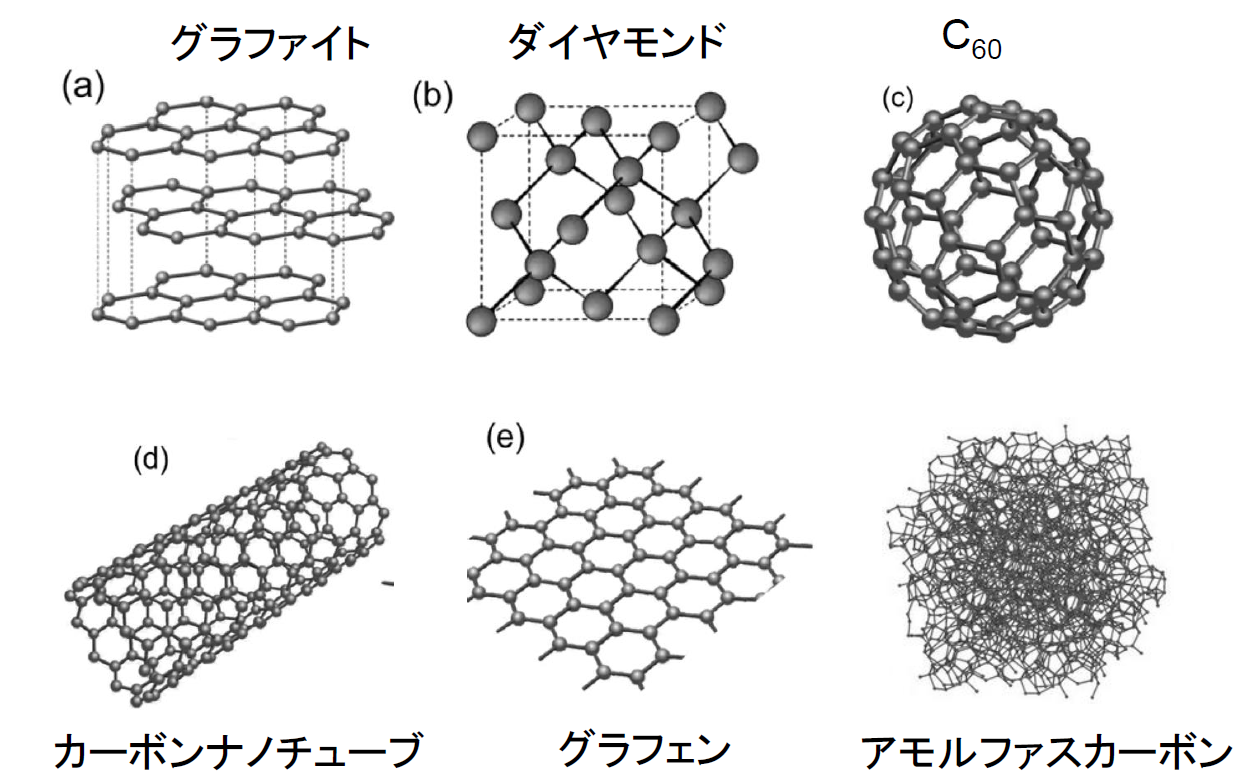
\includegraphics[width=0.8\linewidth]{tester_carbon.png}
  \caption{いろいろな炭素材料}
  \label{fig:tester-carbon}
\end{figure}

鉛筆の芯は，グラファイトと粘土を混ぜ合わせて焼き固めたものです。グラファイトの割合が多いほど芯は柔らかく（B系統），導電性も高くなります。逆に粘土の割合が多いと芯は硬く（H系統），導電性は低くなります。したがって，鉛筆の硬度によって電気の通りやすさが異なります。紙に鉛筆で線を引くと，グラファイトの微小片が紙の表面に付着し，それらが互いに接触して電流の通り道を形成します（\cref{fig:tester-pencil}）。この経路の長さが長くなれば抵抗は大きくなり，幅が広くなれば抵抗は小さくなります。また，塗り方の濃さや重ね塗り，紙の表面の形状の変化によっても，黒鉛片どうしのつながりが変化して抵抗値が変動します。

\begin{figure}[htbp]
  \centering
  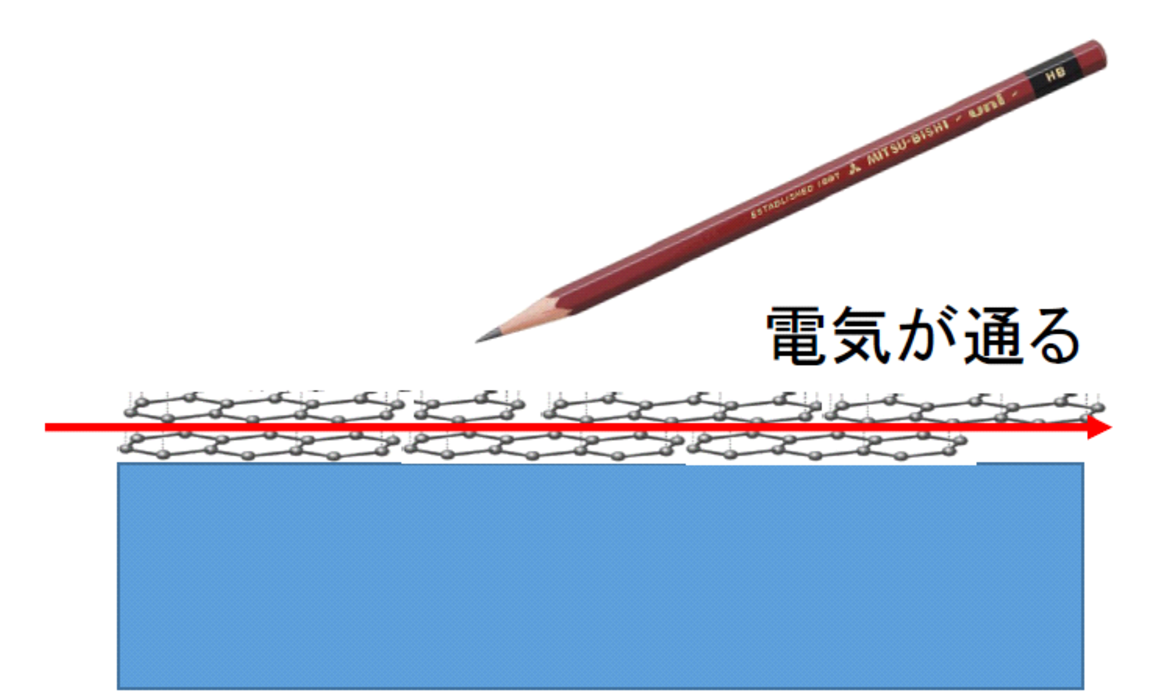
\includegraphics[width=0.5\linewidth]{tester_pencil_line.pdf}\hfill
  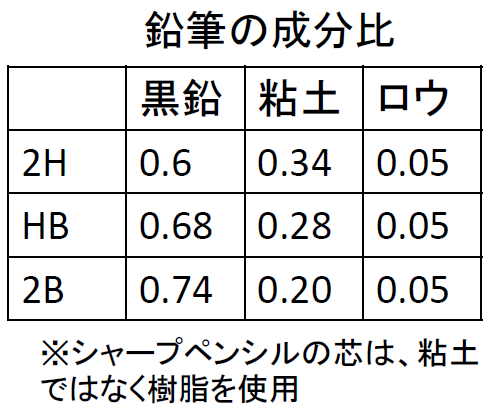
\includegraphics[width=0.42\linewidth]{tester_pencil_composition.png}
  \caption{鉛筆芯の特性}
  \label{fig:tester-pencil}
\end{figure}


% ============================================================
\section{使用器具と使い方}

\begin{equipment}
\begin{itemize}
  \item デジタルテスター
  \item 乾電池・電池ボックス
  \item 抵抗（\SI{100}{\ohm}，\SI{200}{\ohm}，\SI{1}{k\ohm}）
  \item ブレッドボード・リード線
  \item USB充電器，コンセント，ACアダプタ
  \item 鉛筆（2Bなど濃いものが望ましい）
  \item 方眼紙
\end{itemize}
\end{equipment}

% ------------------------------------------------------------
\subsection{デジタルテスターの使い方}

\begin{figure}[htbp]
  \centering
  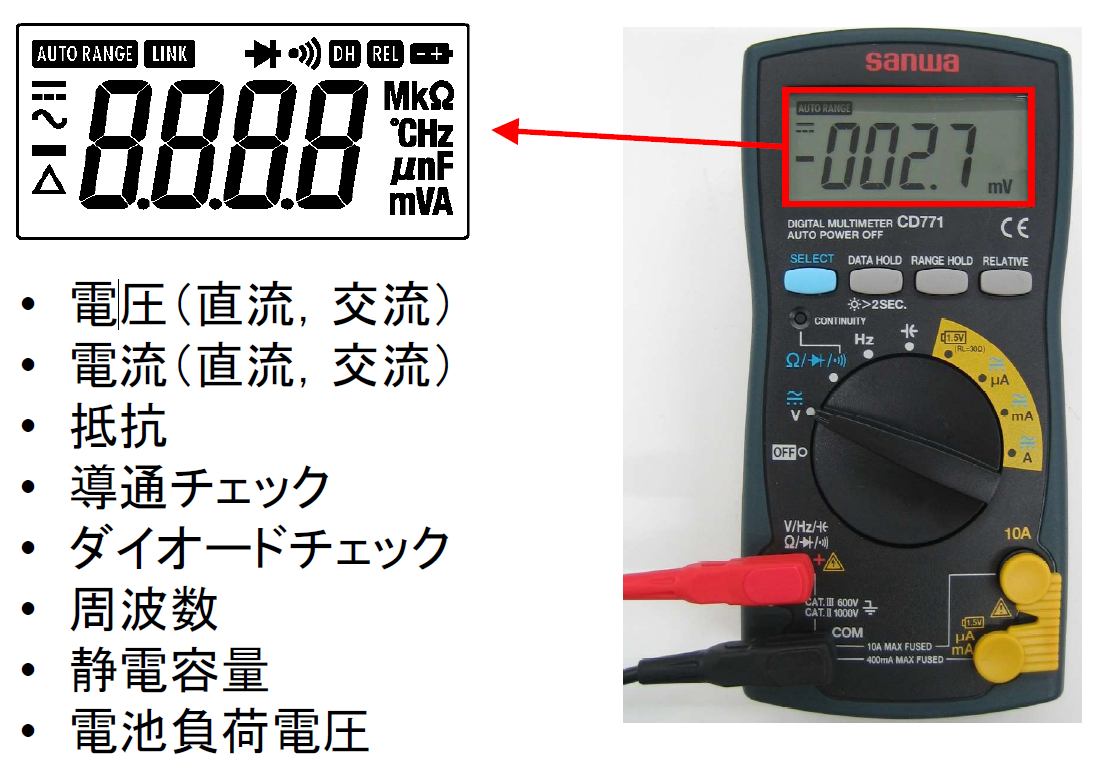
\includegraphics[width=0.72\linewidth]{tester_multimeter.png}
  \caption{デジタルテスター}
  \label{fig:tester-multimeter}
\end{figure}

デジタルテスターは，電気回路の基本的な特性を測定するための装置です。主に電圧（直流・交流），電流（直流・交流），抵抗の測定に用いられるほか，導通チェックやダイオードチェック，静電容量や周波数の測定機能を備えています（\cref{fig:tester-multimeter}）。

\begin{figure}[htbp]
  \centering
  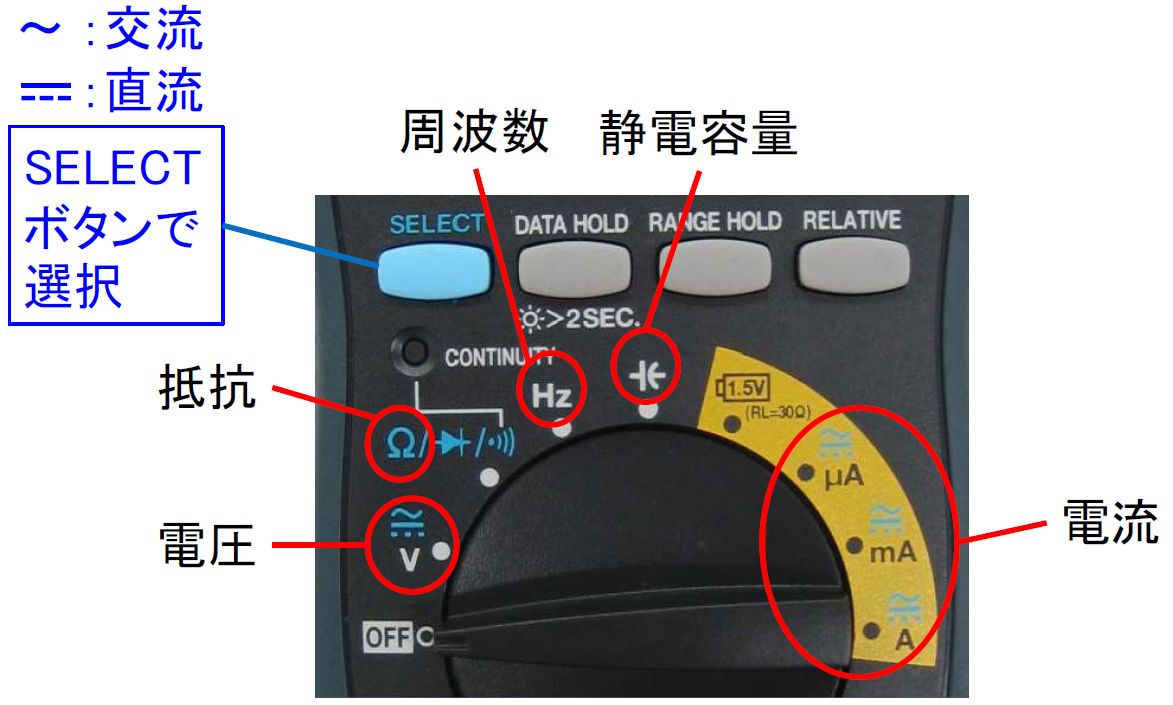
\includegraphics[width=0.72\linewidth]{tester_modes.png}
  \caption{デジタルテスターの測定モード}
  \label{fig:tester-modes}
\end{figure}

本実験では，電圧測定と抵抗測定を中心に使用します。\cref{fig:tester-modes}に示すように，テスターの前面には測定モードを切り替えるためのダイヤルがあり，測定対象に応じて「直流電圧」「交流電圧」「抵抗」などを選択します。直流と交流は表示記号が異なり，直線（―）は直流を，波形（～）は交流を意味します。さらに一部の機種では「SELECT」ボタンを押すことで，同じ測定レンジ内で直流と交流を切り替えることができます。

プローブは赤と黒の2本があり，黒は常に「COM」端子に接続し，赤は測定対象に応じて「V/$\Omega$」端子（電圧・抵抗測定用）や「A」端子（電流測定用）に差し込みます。\wave{誤った端子に差し込んだまま測定すると，ヒューズが切れるなど故障の原因となるため注意が必要です。}測定時には，対象の電気回路の性質に応じて以下の点に注意してください。

\begin{itemize}
  \item \important{電圧測定：}回路を切り離さず，測定したい部分の両端にプローブを当てます。直流の場合は極性（赤がプラス，黒がマイナス）を確認します。
  \item \important{抵抗測定：}\wave{必ず電源を外した状態で行います。}電源が入ったまま抵抗を測定すると誤った値が表示されるだけでなく，テスターを破損させる恐れがあります。また，大きな抵抗値（およそ数百\si{k\ohm}以上）を測定する場合には，テスター内部の構造（内部抵抗）の影響によって正しい値が得られないことがあります。テスターは理想的な計測器ではなく，有限の内部抵抗を持っているためです。これにより実際にどのような誤差が生じるか，また内部抵抗がどのように影響するかについては，2年生で行う電気電子工学実験IIで詳しく取り扱います。
  \item \important{交流測定（コンセント等）：}高電圧を扱うため，\wave{必ず教員の立ち会いのもとで操作し，プローブの金属部分には触れないようにしてください。}
\end{itemize}

このように，デジタルテスターは正しく操作すれば非常に多用途かつ便利な計測器ですが，不注意に扱うと危険や誤測定につながります。したがって，測定対象に合わせたダイヤル設定，端子接続，プローブの扱い方を理解し，安全に使用することが重要です。

% ------------------------------------------------------------
\subsection{ブレッドボードの使い方}

ブレッドボードは，電子回路の試作や学習に広く用いられる基板です。はんだ付けを行わずに部品やリード線を差し込むだけで回路を組むことができるため，初心者でも安全に回路実験を行えるのが特徴です。内部は金属のクリップで構成されており，穴の並び方によって導通の範囲が決まっています。一般的なブレッドボードでは，以下のような規則で電気的に接続されています。

\begin{figure}[htbp]
  \centering
  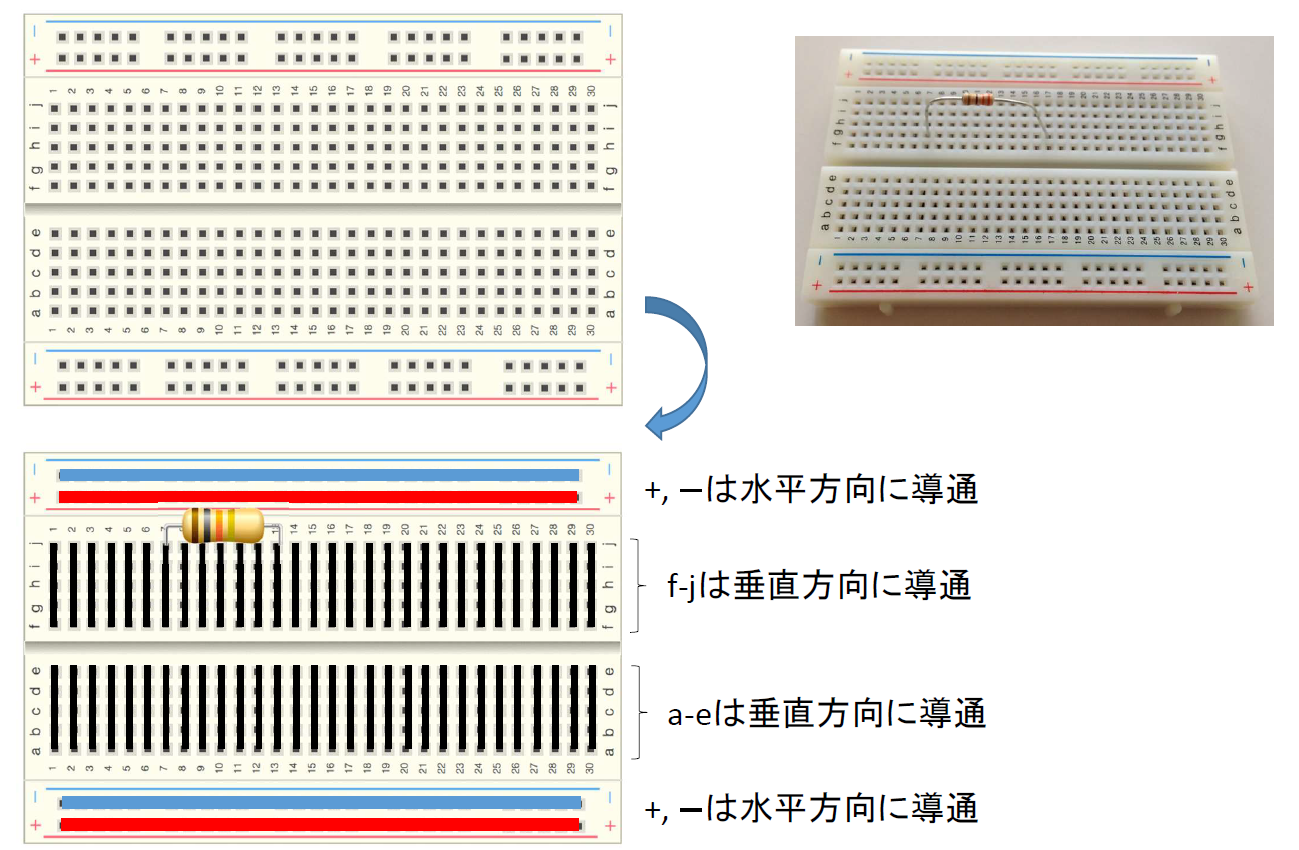
\includegraphics[width=0.8\linewidth]{tester_breadboard.png}
  \caption{ブレッドボード}
  \label{fig:tester-breadboard}
\end{figure}

\begin{itemize}
  % 原文は「図２」だが，ブレッドボードの図を指すため図3（fig:breadboard）に修正
  \item \important{中央部分（\cref{fig:tester-breadboard} a〜e列，f〜j列）：}縦方向に5つの穴がつながっています。ここに抵抗や素子のリードを差し込むと，同じ列内で電気的に接続されます。
  \item \important{両側の電源ライン（$+$，$-$の表示付き）：}横方向に長く連続して導通しています。電源のプラスとマイナスをここに配線しておくことで，どの位置からでも電源を取り出せます。
\end{itemize}

実際に回路を組むときには，乾電池ボックスなどの電源を$+$ラインと$-$ラインに接続し，抵抗やリード線を中央部分に差し込んで回路を構成します。抵抗を直列に接続する場合は，異なる縦列にまたがるように配置し，並列接続にする場合は同じ縦列に差し込みます。

% ------------------------------------------------------------
\subsection{抵抗器の表示}

\begin{figure}[htbp]
  \centering
  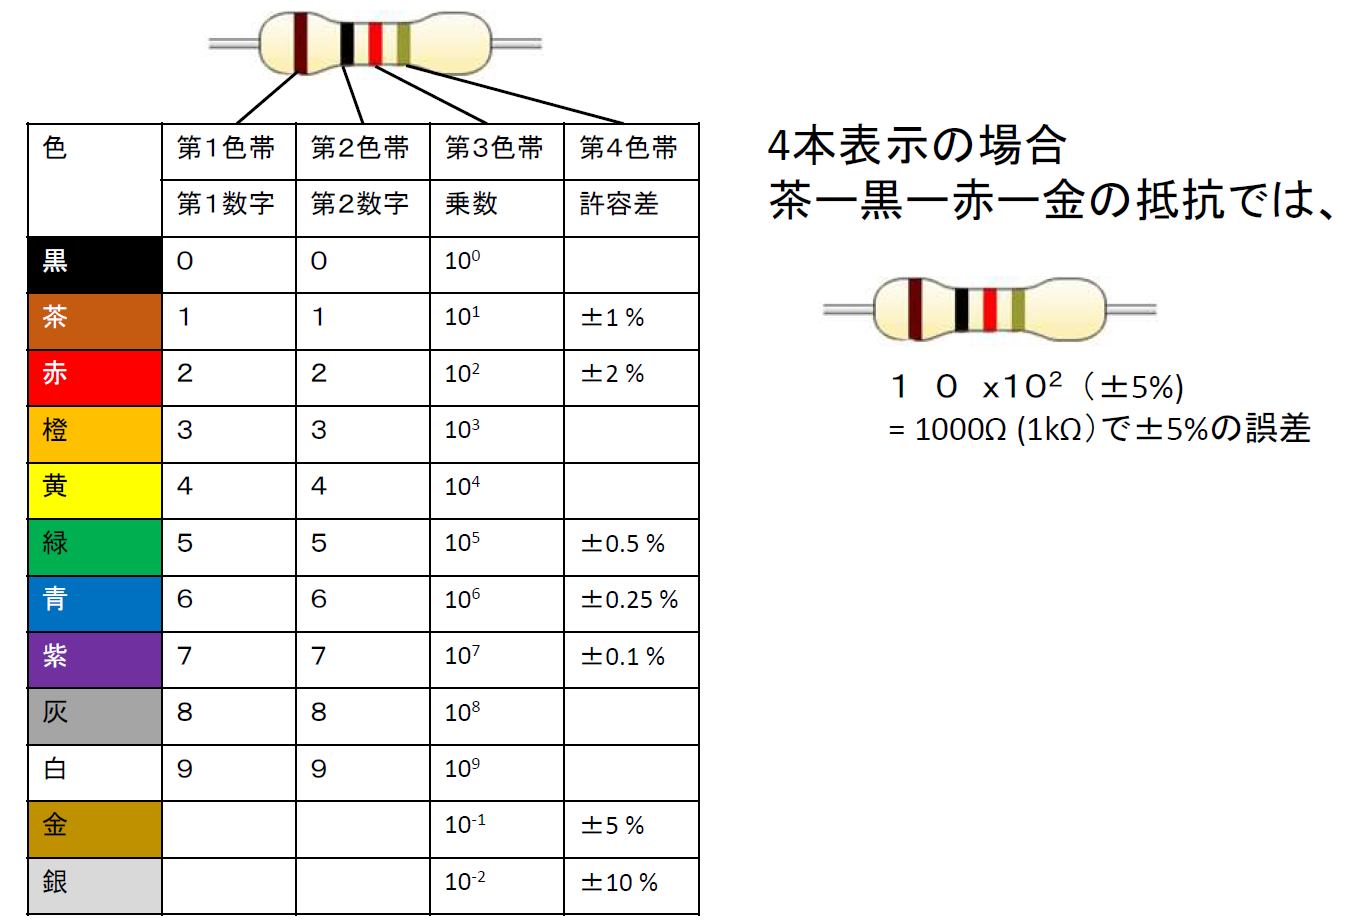
\includegraphics[width=0.8\linewidth]{tester_colorcode.png}
  \caption{カラーコードによる抵抗値の表示方法（JIS C 5062）}
  \label{fig:tester-colorcode}
\end{figure}

市販の抵抗器には抵抗値が印刷されていないものも多く，その場合は「カラーコード」によって値が示されています。\cref{fig:tester-colorcode}に示すように，4本表示の場合には，第1帯および第2帯がそれぞれ抵抗値の第1数字および第2数字を表し，第3帯が乗数（10の何乗を掛けるか），第4帯が許容差（誤差範囲）を表します。例えば「茶--黒--赤--金」の場合は
\begin{itemize}
  \item 第1帯（茶）＝1
  \item 第2帯（黒）＝0
  \item 第3帯（赤）＝$\times 100$
  \item 第4帯（金）＝許容差 $\pm\SI{5}{\percent}$
\end{itemize}
となり，抵抗値は $10\times 100 = \SI{1000}{\ohm}$（\SI{1}{k\ohm}）$\pm\SI{5}{\percent}$ となります。実験では，\SI{100}{\ohm}，\SI{200}{\ohm}，\SI{1}{k\ohm}の抵抗を使用します。

% ============================================================
\section{実験方法}

% ------------------------------------------------------------
\subsection{実験1：身近な電圧を測る}

\begin{procedure}[label=\textbf{1.\arabic*}, ref=1.\arabic*, leftmargin=*, labelsep=0.8em]
  \item テスターを直流電圧（DCV）に設定し，黒プローブをCOM，赤プローブをV/$\Omega$端子へ接続します。
  \item \important{乾電池：}電池ボックスの$+$と$-$にプローブを当て，端子電圧 $V_0$ を測定します。
  \item \important{USBポート：}通常のUSBコネクタは端子間が狭く，\wave{テスターのプローブを直接当てるとショートの危険があります。}そのため，本実験では，あらかじめ準備した「測定用USBケーブル」を使用し，端子部分にプローブを当てて，USB電圧を測定します。
  \item \important{ACアダプタ：}ACアダプタの出力端子にプローブを当て，出力電圧を測定します。
  \item \important{コンセント（AC）：}テスターを交流電圧（ACV）に切り替えます（プローブ端子の差し替えは不要です）。\wave{教員立会いのもと}，商用電源の電圧を測定します。
\end{procedure}

% ------------------------------------------------------------
\subsection{実験2：負荷をつないだときの電圧}

\begin{procedure}[label=\textbf{2.\arabic*}, ref=2.\arabic*, leftmargin=*, labelsep=0.8em]
  \item テスターを直流電圧（DCV）に戻します。
  \item ブレッドボード上で乾電池と\SI{1}{k\ohm}の抵抗を直列に接続し，乾電池の両端の電圧 $V_{1\,\mathrm{k\Omega}}$ を測定します。
  \item 抵抗を\SI{200}{\ohm}や\SI{100}{\ohm}に取り替え，同様に乾電池の両端の電圧 $V_{200\,\Omega}$ および $V_{100\,\Omega}$ をそれぞれ測定します。
  \item それぞれの抵抗値・電圧値をまとめます。さらに，抵抗値から電流を計算し，電流と電圧の関係を確認します。
\end{procedure}

% ------------------------------------------------------------
\subsection{実験3：鉛筆で書いた線の長さ・幅と抵抗値の関係}

\begin{figure}[htbp]
  \centering
  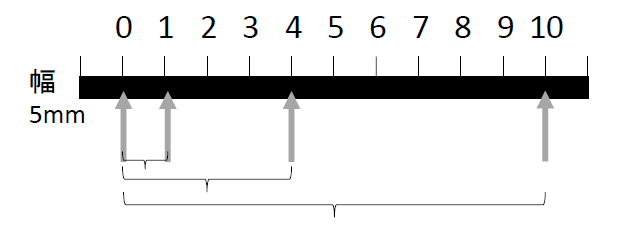
\includegraphics[width=0.47\linewidth]{tester_expC_5mm.png}\hfill
  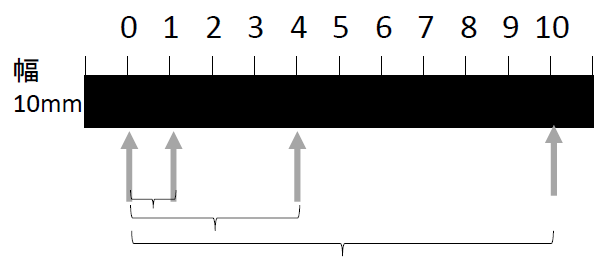
\includegraphics[width=0.47\linewidth]{tester_expC_10mm.png}
  \caption{鉛筆で書いた線の長さ・幅と抵抗値の関係の実験}
  \label{fig:tester-exp3}
\end{figure}

\begin{procedure}[label=\textbf{3.\arabic*}, ref=3.\arabic*, leftmargin=*, labelsep=0.8em]
  \item テスターを抵抗測定（$\Omega$）に設定し，黒プローブをCOM，赤プローブをV/$\Omega$端子へ接続します（プローブの差し替えは不要です）。
  \item 方眼紙に鉛筆で，線幅\SI{5}{mm}，長さ\SI{12}{cm}の線を書き，内部を濃く，均等に塗りつぶします（\cref{fig:tester-exp3}左）。
  \item 長さ\SI{12}{cm}のうち内部\SI{10}{cm}の部分について，\SI{1}{cm}ごとに長さと抵抗の関係を測定します。この際，塗りムラや濃さにより抵抗値が変わり得るので，測定値を観察しながら必要に応じて線を塗り足すなど工夫してかまいません。
  \item 次に，線幅を\SI{10}{mm}として同様の実験を行います（\cref{fig:tester-exp3}右）。
\end{procedure}

% ------------------------------------------------------------
\subsection{実験4：鉛筆で書いた線の曲げ方向と抵抗値の関係}

\begin{figure}[htbp]
  \centering
  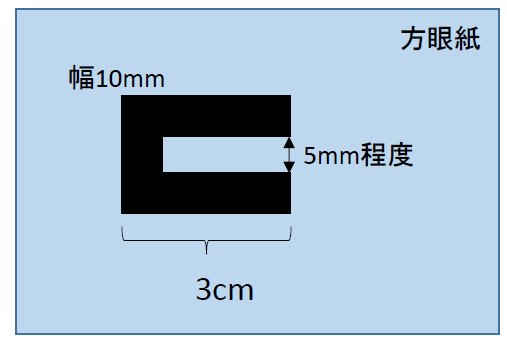
\includegraphics[width=0.47\linewidth]{tester_expD_cut.png}\hfill
  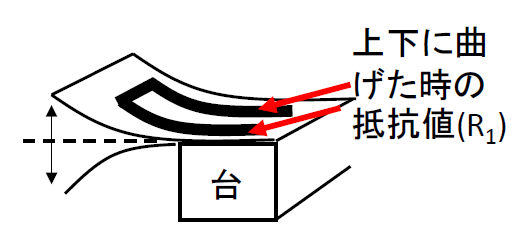
\includegraphics[width=0.47\linewidth]{tester_expD_bend.png}
  \caption{鉛筆で書いた線の曲げ方向と抵抗値の関係の実験}
  \label{fig:tester-exp4}
\end{figure}

\begin{procedure}[label=\textbf{4.\arabic*}, ref=4.\arabic*, leftmargin=*, labelsep=0.8em]
  \item 方眼紙に鉛筆で，幅\SI{10}{mm}，間隔\SI{5}{mm}，長さ\SI{3}{cm}程度のコ字型の図形を書き，内部を塗りつぶします（\cref{fig:tester-exp4}左）。
  \item コ字部分が入った部分を切り抜きます。
  \item コ字をまっすぐ伸ばし，コ字両端部で測定した抵抗値 $R_0$ を記録します。
  \item 次に，机の端や台などを使用して，コ字部分を上下方向に曲げられるようにして，上下に曲げた時の抵抗値 $R_1$，$R_2$ を測定します（\cref{fig:tester-exp4}右）。
\end{procedure}

% ============================================================
\section{考察と課題}

\subsection{乾電池の特性について（実験1・2）}

実験1および実験2の結果から，乾電池から出力する電流の大きさと電圧の関係をグラフにまとめてください。得られたデータに対して最小二乗法を用いて近似直線を引き，その結果から\cref{fig:tester-battery}を参考に乾電池の等価回路を作成してください。

\subsection{鉛筆で書いた線の抵抗値について（実験3）}

鉛筆で描いた線について，長さと抵抗値の関係をグラフにまとめてください。得られたデータに対して最小二乗法を用いて近似直線を引き，線幅および長さと抵抗値の関係を考察してください。それらが比例関係にない場合，その理由を考察してください。

\subsection{線の曲げと抵抗値の関係について（実験4）}

鉛筆で描いたコ字型の線を曲げる前後の抵抗値の変化率 $(R_1-R_0)/R_0$（\si{\percent}）を計算してください。曲げ方向（引っ張り方向・圧縮方向）によって抵抗がどのように変化したかを整理し，黒鉛粒子の接触状態の変化など，背後でどのような物理的現象が起きているかを考察してください。また，この現象がどのような応用に利用できるかを考えてください。

% ============================================================
\section{レポート提出}

% TODO(原文確認): 提出曜日が「〇曜日」のまま
実験の翌週の〇曜日の13:00までにPDFファイルをユニバーサルパスポートで提出してください。

% ============================================================
% 交流回路（オシロスコープを用いた測定） 本文
% 原本: 実験手引書_交流回路(オシロスコープを用いた測定).docx（である調 → です・ます調に変更）
% 担当の先生はこのファイルと figures/ だけを編集してください。
% 図のラベルは fig:oscilloscope-○○ の形にしてください（他テーマとの重複防止）。
% ============================================================
\graphicspath{{contents/02_oscilloscope/figures/}}

\experimenttitle{交流回路（オシロスコープを用いた測定）}

% ============================================================
\section{目的}

オシロスコープの使い方を習得し，基本的なフィルタ回路の動作原理を理解します。

% ============================================================
\section{実用例（音源(PC)から高音成分を除去し，スピーカーから出る音で確認）}

フィルタ回路の1つにローパスフィルタがあります。この回路は高い周波数成分を遮断する機能を有するため，音楽などに含まれる高音成分を取り除くことが可能です。

% ============================================================
\section{原理}

% ------------------------------------------------------------
\subsection{交流}

交流（AC: Alternating Current）とは，時間経過とともに大きさと向きが周期的に変化するものです。典型的な交流波形を図\ref{fig:oscilloscope-waveforms}に示します。

\begin{figure}[htbp]
  \centering
  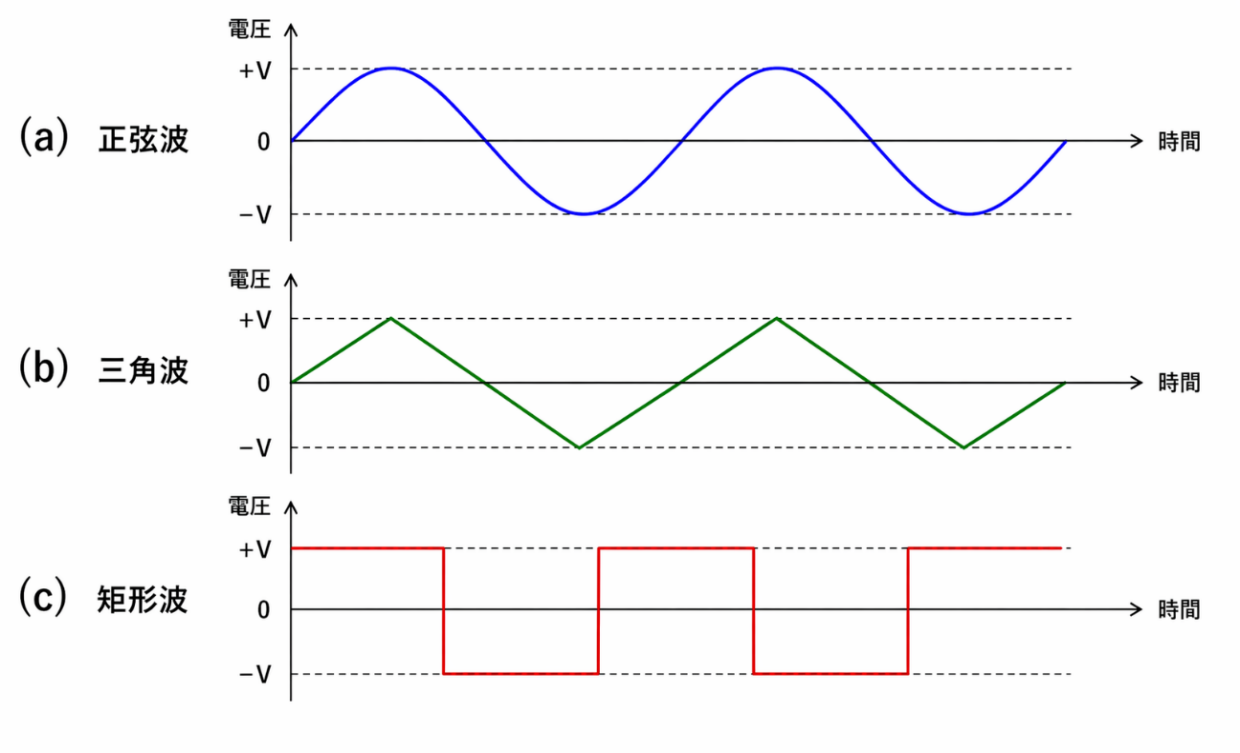
\includegraphics[width=0.7\linewidth]{oscilloscope_waveforms.png}
  \caption{交流波形の例}
  \label{fig:oscilloscope-waveforms}
\end{figure}

図\ref{fig:oscilloscope-waveforms}(a)は正弦波（sinusoidal wave），(b)は三角波（triangular wave），(c)は方形波（または矩形波）（rectangular wave）と呼ばれます。図\ref{fig:oscilloscope-waveforms}(a)のように電圧，電流の大きさが正弦波状に変化するものを正弦波交流といい，交流波形のなかでも最も基本となる波形です。

\begin{figure}[htbp]
  \centering
  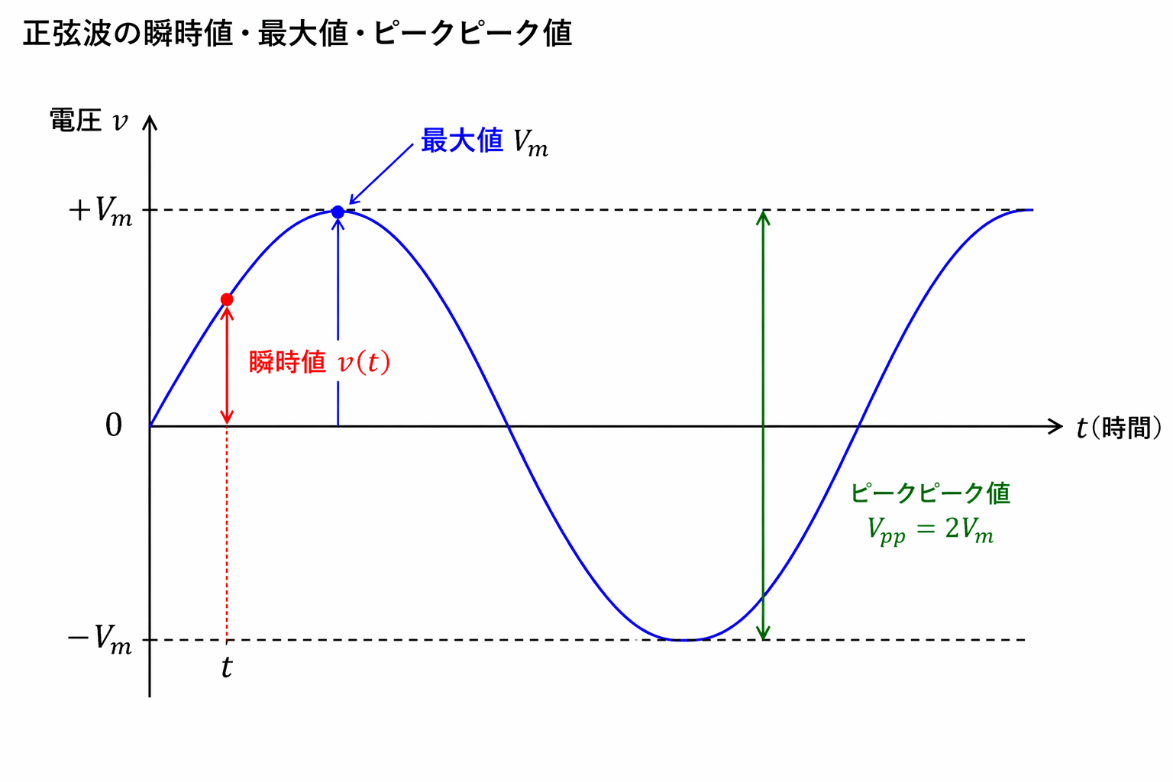
\includegraphics[width=0.7\linewidth]{oscilloscope_instantaneous.png}
  \caption{瞬時値と最大値}
  \label{fig:oscilloscope-instantaneous}
\end{figure}

図\ref{fig:oscilloscope-instantaneous}に示すように交流の任意の時間 $t$ における電圧・電流の値を「瞬時値（instantaneous value）」といいます。瞬時値は電圧の場合には $v$ と表され，電流の場合は $i$ で表されます。瞬時値のなかでも絶対値が最も大きいものを「最大値（maximum value）」といいます。最大値は電圧の場合は $V_\mathrm{m}$ で，電流の場合は $I_\mathrm{m}$ で表されます。最大値のことを「振幅（amplitude）」ともいいます。また，最大値と最小値の差を「ピークピーク値（peak-to-peak value）」といいます。ピークピーク値は電圧の場合 $V_\mathrm{pp}$，電流の場合 $I_\mathrm{pp}$ で表されます。交流の瞬時電圧は一般的にはオシロスコープ（oscilloscope）を用いて測定します。オシロスコープとは，電気信号（電圧）の時間経過に対する変動を測って波形として画面に表示して観測する測定器です。

% ------------------------------------------------------------
\subsection{$RC$回路（ローパスフィルタ）}

% TODO(原文確認): 見出し・本文は RC ローパスフィルタだが，図は LC ローパスフィルタ（原本のまま）
\begin{figure}[htbp]
  \centering
  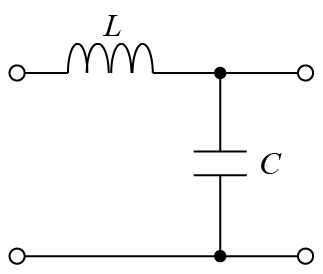
\includegraphics[width=0.35\linewidth]{oscilloscope_lc_lowpass.png}
  \caption{$LC$ローパスフィルタの回路図}
  \label{fig:oscilloscope-lc-lowpass}
\end{figure}

$RC$ローパスフィルタは，低い周波数は通して，高い周波数は通しにくくする回路です。$RC$ローパスフィルタは，抵抗（$R$）とコンデンサ（$C$）を組み合わせて構成されます。低い周波数成分を通し，高い周波数成分を減衰させる回路です。出力は一般的にコンデンサの両端から取り出されます。コンデンサは周波数が低いと電流を流しにくく，周波数が高いと電流を流しやすいという性質を持つため，低周波信号では出力電圧がほぼそのまま保持されます。一方，高周波信号では電流がコンデンサを通って接地側へ流れやすくなり，出力電圧が小さくなります。この性質により，高周波のノイズを除去し，滑らかな電圧波形を得ることができます。\important{周波数特性の境目となる周波数はカットオフ周波数と呼ばれ}，その値は
\begin{equation}
  f_\mathrm{c} = \frac{1}{2\pi RC}
  \label{eq:oscilloscope-cutoff}
\end{equation}
で表されます。$RC$ローパスフィルタは，ノイズ除去，平滑回路など電子回路やパワーエレクトロニクス分野で広く利用されています。

% ------------------------------------------------------------
\subsection{$RLC$直列共振フィルタ回路}

\begin{figure}[htbp]
  \centering
  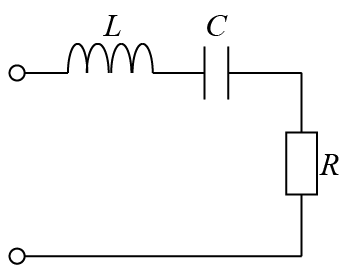
\includegraphics[width=0.35\linewidth]{oscilloscope_rlc_series.png}
  \caption{$RLC$直列共振の回路図}
  \label{fig:oscilloscope-rlc-series}
\end{figure}

交流回路では，抵抗は周波数が変化しても影響はありませんが，コイル $L$ やコンデンサ $C$ は周波数の変化に伴い，性質が変化します。コイルは周波数が高くなるほど電流を流しにくくなり，コンデンサは逆に周波数が高くなると電流を流しやすくなります。また，ある特定の周波数になると，コイルとコンデンサのリアクタンスが等しくなります。この状態を\important{共振}といい，\important{共振周波数} $f_0$ は
\begin{equation}
  f_0 = \frac{1}{2\pi\sqrt{LC}}
  \label{eq:oscilloscope-resonance}
\end{equation}
で表せます。

% ------------------------------------------------------------
\subsection{カットオフ周波数}

% 原文は「f_c = 1/√2 ≈ 0.707 となる周波数」。f_c の式ではなく出力電圧の比の意味なので書き換え（要確認）
カットオフ周波数 $f_\mathrm{c}$ とは，フィルタ回路が信号を通す領域と\important{減衰させる領域の境界となる周波数}です。一般的に，出力電圧が最大値の $1/\sqrt{2}\approx 0.707$ 倍となる周波数として定義されます（図\ref{fig:oscilloscope-lowpass-response}）。

\begin{figure}[htbp]
  \centering
  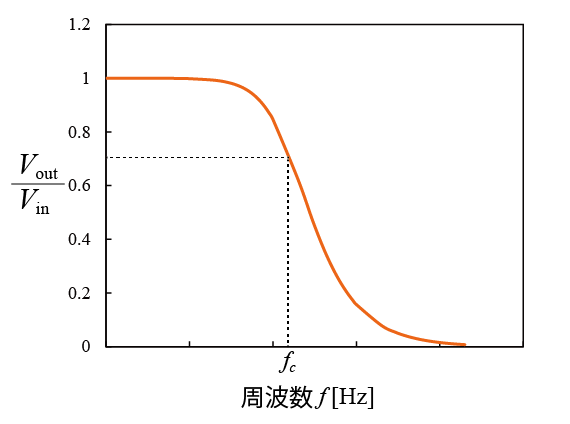
\includegraphics[width=0.5\linewidth]{oscilloscope_lowpass_response.png}
  \caption{ローパスフィルタの周波数特性}
  \label{fig:oscilloscope-lowpass-response}
\end{figure}

% ============================================================
\section{使用器具}

\begin{equipment}
\begin{itemize}
  \item オシロスコープ
  \item 交流電源（信号発生器）
  % TODO(原文確認): 実験2では 10 Ω の抵抗を使うが，ここには 100 Ω とある
  \item 抵抗（\SI{100}{\ohm}×1，\SI{1}{k\ohm}×1）
  \item コンデンサ（\SI{0.1}{\micro F}×1，\SI{1}{\micro F}×1）
  \item コイル（\SI{10}{mH}×1）
  \item ブレッドボード，ジャンパ線
\end{itemize}
\end{equipment}

% ============================================================
\section{実験方法}

測定結果は，ワークシートの表に記録してください。

% ------------------------------------------------------------
\subsection{実験1：$RC$ローパスフィルタの特性}

\begin{figure}[htbp]
  \centering
  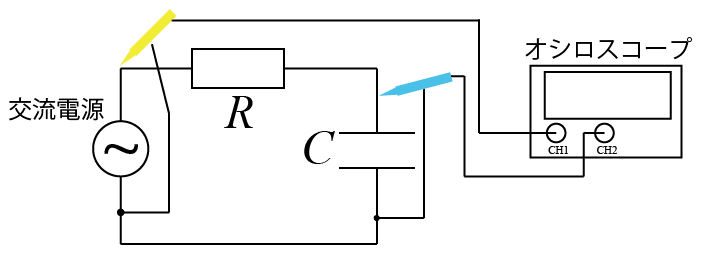
\includegraphics[width=0.75\linewidth]{oscilloscope_circuit1.png}
  \caption{測定回路1}
  \label{fig:oscilloscope-circuit1}
\end{figure}

\begin{procedure}[label=\textbf{1-\arabic*}, leftmargin=*, labelsep=0.8em]
  % 原文は「図4に示すような回路」だが測定回路1（図6）を指すと判断
  \item 図\ref{fig:oscilloscope-circuit1}に示すような回路を作製し，交流源（信号発生器）の周波数を変化させて出力電圧の最大値を測定します。ここで，交流電源の電圧を\SI{10}{V}に設定します。素子は抵抗\SI{1}{k\ohm}（茶黒赤金），コンデンサ\SI{1}{\micro F}を使用します。周波数は\SI{20}{Hz}～\SI{1}{kHz}まで変化させ，周波数特性を記録します。オシロスコープのCH1（黄）には入力波形，CH2（青）には出力波形を表示します。表示される波形の最大値 $V_\mathrm{m}$ を記録してください。\\
    ※Excelを用いてグラフを作成します。
  \item カットオフ周波数 $f_\mathrm{c}$ を確認します。
  \item 自作したローパスフィルタをPC（音源）とスピーカーに接続して機能を確認します。
\end{procedure}

% ------------------------------------------------------------
\subsection{実験2：$RLC$直列共振フィルタの特性}

\begin{figure}[htbp]
  \centering
  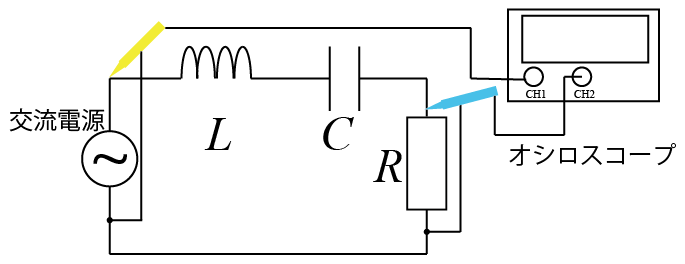
\includegraphics[width=0.75\linewidth]{oscilloscope_circuit2.png}
  \caption{測定回路2}
  \label{fig:oscilloscope-circuit2}
\end{figure}

\begin{procedure}[label=\textbf{2-\arabic*}, leftmargin=*, labelsep=0.8em]
  % 原文は「図5に示すような回路」だが測定回路2（図7）を指すと判断
  \item 図\ref{fig:oscilloscope-circuit2}に示すような回路を作製し，交流源（信号発生器）の周波数を変化させて出力電圧の最大値を測定します。ここで，交流電源の電圧を\SI{10}{V}に設定します。素子は抵抗\SI{10}{\ohm}（茶黒黒金），コイル\SI{10}{mH}，コンデンサ\SI{0.1}{\micro F}を使用します。周波数は\SI{2}{kHz}～\SI{8}{kHz}まで変化させ，周波数特性を記録します。オシロスコープのCH1（黄）には入力波形，CH2（青）には出力波形を表示します。CH2に表示される波形の最大値 $V_\mathrm{m}$ を記録してください。\\
    ※Excelを用いてグラフを作成します。
  \item 測定した結果から共振周波数を確認します。
\end{procedure}

% ============================================================
% ダイオードを用いた電子回路 本文
% 担当の先生はこのファイルと figures/ だけを編集してください。
% 図のラベルは fig:diode-○○ の形にしてください（他テーマとの重複防止）。
% ============================================================
\graphicspath{{contents/03_diode/figures/}}

\experimenttitle{ダイオードを用いた電子回路}

% ============================================================
\section{目的}

発光ダイオード（LED：Light Emitting Diode）の整流性を確認し，発光色の異なるLEDの点灯と電圧の関係を調べます。また，ダイオードの整流性を利用した整流回路について出力波形の変化を調べます。

% ============================================================
\section{ダイオードについて}

ダイオードは，電流を一方向にのみ流す電子部品です。電気の流れをコントロールする「電気の逆流防止弁」のような働きをします。ダイオードは，P型半導体とN型半導体が接合した構造をしており，この接合面をPN接合と呼びます。

\begin{figure}[htbp]
  \centering
  \begin{minipage}[b]{0.46\linewidth}
    \centering
    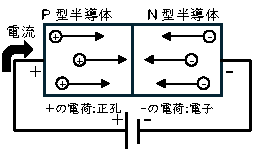
\includegraphics[scale=1.3]{diode_pn_forward.pdf}
    \caption{順方向電圧を印加}
    \label{fig:diode-pn_forward}
  \end{minipage}
  \hfill
  \begin{minipage}[b]{0.46\linewidth}
    \centering
    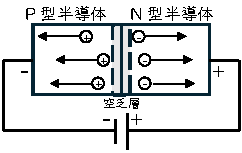
\includegraphics[scale=1.3]{diode_pn_reverse.pdf}
    \caption{逆方向電圧を印加}
    \label{fig:diode-pn_reverse}
  \end{minipage}
\end{figure}

図\ref{fig:diode-pn_forward}に示すように，P型半導体側にプラス，N型半導体側にマイナスの電圧（順方向電圧）を印加すると，PN接合部分で，正の電荷（正孔）と負の電荷（電子）が再結合して電流が流れます。一方，図\ref{fig:diode-pn_reverse}に示すようにP型半導体側にマイナス，N側半導体側にプラスの電圧（逆方向電圧）を印加するとPN接合の部分に電荷が存在しない空乏層が形成され，電流は流れません。この性質を利用して，様々な電子機器に利用されています。

\subsection{ダイオードの種類}

ダイオードには様々な種類があり，それぞれ異なる用途で使用されています。

\begin{enumerate}
  \item \keyword{発光ダイオード（LED）}\quad ※本実験では，LEDを用いた実験を行います。\\
    順方向に電圧を印加すると発光します。LEDの材料によって，発光色や光り始める電圧が異なります。信号機，照明，ディスプレイなど，現代の生活に欠かせない部品の1つです。
  \item \keyword{整流ダイオード}\\
    交流を直流に変換する整流回路に特化した素子です。LEDよりも大きな電流を扱うことができ，家電製品の電源回路など，幅広い電子機器で使用されています。
  \item \keyword{ツェナーダイオード}\\
    逆方向に一定以上の電圧（ツェナー電圧）を印加しても電流が流れる性質を持ちます。電圧を一定に保つ定電圧回路に使用されます。
  \item \keyword{フォトダイオード}\\
    光を受けると電流を流す受光素子で，光センサー等に使用されます。出力電力に特化したものが太陽電池になります。
\end{enumerate}

\subsection{LED}

\begin{figure}[htbp]
  \centering
  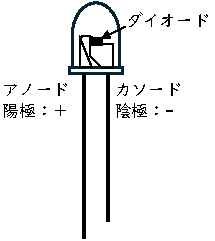
\includegraphics[scale=1.3]{diode_led_appearance.pdf}
  \caption{LEDの外観図}
  \label{fig:diode-led}
\end{figure}

図\ref{fig:diode-led}に砲弾型のLEDの外観図を示します。金属線が長いほうがアノード（陽極：$+$），足が短いほうがカソード（陰極：$-$）となります。金属線の長さに違いがない場合は，LEDの発光部を横から見て判別します。ダイオードが乗っていない側（図\ref{fig:diode-led}では左側）がアノード，ダイオードが乗っている側（図\ref{fig:diode-led}では右側）がカソードとなります。LEDに順方向電圧を印加するとPN接合の部分で正孔と電子が再結合して電流が流れて発光します。LEDの発光色は使用されているダイオードの材料によって異なります。赤色にはアルミニウムガリウムヒ素（AlGaAs）やガリウムヒ素リン（GaAsP）など，黄緑色には窒化インジウムガリウム（InGaN）など，青色には窒化ガリウム（GaN）などが用いられています。

% ============================================================
\section{使用器具}

\begin{equipment}
\begin{itemize}
  \item LED（赤色6個，黄緑色1個，青色1個，白色1個）\quad ※接続時，極性（向き）に注意
  \item 固定抵抗器 $R$（\SI{100}{\ohm}/\SI{1}{W}，\SI{1}{\mega\ohm}/\SI{0.25}{W}）\quad ※極性（向き）はありません
  \item セラミックコンデンサー $C$（\SI{10}{\micro F}）1個\quad ※極性（向き）はありません
  \item ブレッドボード 1個
  \item ジャンパー線 必要数
  \item 直流電源 1台\quad ※接続時，極性（向き）に注意
  \item 交流電源 1台\quad ※接続時，極性（向き）に注意
  \item オシロスコープ 1台
  \item オシロスコープのプローブ 2本
\end{itemize}
\end{equipment}

% ============================================================
\section{実験方法}

% ------------------------------------------------------------
\subsection{実験1：LEDの整流性の確認と赤色LEDの点灯実験}

赤色LEDの整流性を確認するため，逆方向接続もしくは順方向接続して電圧印加時の赤色LEDの点灯状態を確認します。

\begin{figure}[htbp]
  \centering
  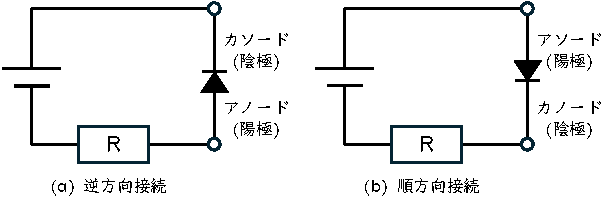
\includegraphics[scale=1.3]{diode_exp1_circuit.pdf}
  \caption{実験1の回路図}
  \label{fig:diode-exp1}
\end{figure}

\begin{procedure}[label=\textbf{(\alph*)}]
  \item \keyword{逆方向接続}\\
    LEDの極性（アノードとカソードの向き）に気を付けて，逆方向電圧を印加する回路をブレッドボード上に作製します（図\ref{fig:diode-exp1}(a)逆方向接続）。固定抵抗器 $R$（\SI{100}{\ohm}/\SI{1}{W}）は，LEDに電流が流れすぎないようにするために用います。出力をONした後，直流電源の電圧を\SI{0}{V}から\SI{3}{V}（実際には直流電源を逆に接続するため回路には\SI{0}{V}から\SI{-3}{V}）までゆっくりと印加し，直流電源に表示される電流と赤色LEDの発光状態を確認します。\wave{発光しないことを確認後，電圧を\mbox{\SI{0}{V}}にもどし，出力をOFFします。}
  \item \keyword{順方向電圧}\\
    LEDの極性に気を付けて，順方向電圧を印加する回路をブレッドボード上に作製します（図\ref{fig:diode-exp1}(b)順方向接続）。出力をONした後，直流電源の電圧を\SI{0}{V}からゆっくりと印加し，直流電源に表示される電流表示が\SI{0.001}{A}となるときの電圧 $V$（V）を読み取り，課題1の表に記載します。\wave{発光確認後，電圧を\mbox{\SI{0}{V}}にもどし}，\wave{出力をOFFします。}
\end{procedure}

% ------------------------------------------------------------
\subsection{実験2：様々なLEDの点灯実験}

異なる色のLEDが点灯する電圧（電流表示が\SI{0.001}{A}になる）を調べます。

LED（黄緑色LED，青色LED，白色LED）の極性に気を付けて順方向電圧を印加する回路をブレッドボード上に作製します（図\ref{fig:diode-exp1}(b)順方向接続）。出力をONした後，直流電源の電圧を\SI{0}{V}からゆっくりと印加し，電源電圧の電流表示が\SI{0.001}{A}となるとき，各LEDの電圧 $V$（V）を読み取り，課題1の表に記載します。\wave{発光確認後，電圧を\mbox{\SI{0}{V}}にもどし}，\wave{出力をOFFします。}
% TODO(原文確認): 次の文は原文のまま。意味が通らないため要修正
\wave{LEDを交換し，}\wave{電圧の出力とで電圧に気を付けLEDが点灯する電圧を調べます。}

% ------------------------------------------------------------
\subsection{実験3：赤色LEDの整流性を利用した電圧波形の変化}

LEDの整流性を利用し，正弦波交流波形の変化を観測します。

\subsubsection{オシロスコープの準備}

\begin{procedure}
  \item オシロスコープに電源ケーブルを接続し，主電源を入れてオシロスコープが起動するのを待ちます。
  \item 起動後，「Default Setup」ボタンを押し，オシロスコープの設定を初期化します。初期化によって電圧軸は\SI{5.00}{V}/DIV，時間軸は\SI{100.0}{\micro s}/DIVに設定されます。
  \item CH1にオシロスコープのプローブを接続し，CH1の測定端子をオシロスコープのDemo端子に接続します。
  \item 「Auto Scale」ボタンを押すと，電圧軸は\SI{500}{mV}/DIV，時間軸は\SI{200.0}{\micro s}/DIVに設定され，Demo端子からの波形が表示されます。
  \item 「Meas」ボタンを押すと，Demo端子からの出力波形の周波数がおよそ\SI{1}{kHz}，p-pがおよそ\SI{2.5}{V}であることがわかります。
  \item オシロスコープのCH1とCH2の接続部分の上部に記載されています「押してゼロ設定」の「右側のノブ」を押すと，基準電圧が中央に移動します。
  \item 垂直軸をまわして電圧を\SI{2.00}{V}/DIV，水平軸をまわして時間を\SI{200.0}{ms}/DIVに設定します。
\end{procedure}

\subsubsection{交流電源の準備}

\begin{figure}[htbp]
  \centering
  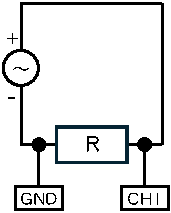
\includegraphics[scale=1.3]{diode_ac_setup.pdf}
  \caption{交流電源設定回路}
  \label{fig:diode-ac_setup}
\end{figure}

\begin{procedure}
  \item 交流電源に電源ケーブルを接続し，出力ケーブルを接続します。
  \item 交流電源のAMPLが最小値（反時計回りに回りきっている状態），ATTが押されていない状況を確認し，交流電源をONします。
  \item 周波数を\SI{2}{Hz}（x20のボタンを押し，\SI{0.0020}{kHz}表示），正弦波形のボタンを押します。
  \item ブレッドボード上に図\ref{fig:diode-ac_setup}の回路（固定抵抗 $R$（\SI{100}{\ohm}/\SI{1}{W}））を作製し，オシロスコープのCH1のプローブを図\ref{fig:diode-ac_setup}のように接続します。
  \item 交流電源のAMPLをゆっくりと増加（時計回りに回す）させ，オシロスコープのp-pがおよそ\SI{12.0}{V}となるように設定し，「トリガ」を回し，トリガの位置を\SI{2.00}{V}にします。
  % 原文はSymbolフォントで「200 μs/DIV」。2 Hzの観測なので ms と判断（要確認）
  \item オシロスコープで観察される電圧波形を課題2の図(a)に図示してください。（オシロスコープの表示設定は\SI{2.00}{V}/DIV，\SI{200}{ms}/DIVとなっています。）
  \item 観察終了後，交流電源の電源をOFFにします。
\end{procedure}

\subsubsection{LEDを用いた点灯実験}

\begin{figure}[htbp]
  \centering
  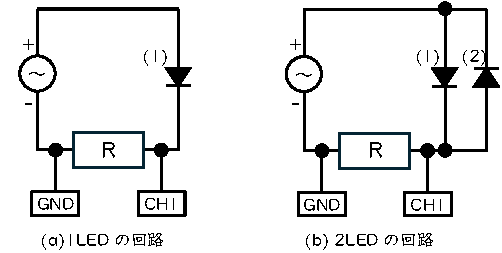
\includegraphics[scale=1.3]{diode_led_ac.pdf}
  \caption{LEDを用いた点灯実験}
  \label{fig:diode-led_ac}
\end{figure}

\begin{procedure}
  \item LEDの極性に気を付けて図\ref{fig:diode-led_ac}(a)に示す回路をブレッドボード上に作製します。
  \item オシロスコープのCH1のプローブを図\ref{fig:diode-led_ac}(a)のように接続したのち，交流電源をONにして，LED(1)の点灯状態とオシロスコープで抵抗器 $R$ の電圧波形を確認します。（LED(1)が点滅します。）
  \item 確認後，交流電源の電源をOFFにします。
  \item LEDの極性に気を付けて図\ref{fig:diode-led_ac}(b)に示す回路をブレッドボード上に作製します。
  \item 交流電源をONにして，LEDの点灯状態とオシロスコープで抵抗器 $R$ の電圧波形を確認します。（LED(1)とLED(2)が交互に点灯します。）
  \item 確認後，交流電源をOFFにします。
\end{procedure}

\subsubsection{整流回路1}

\begin{figure}[htbp]
  \centering
  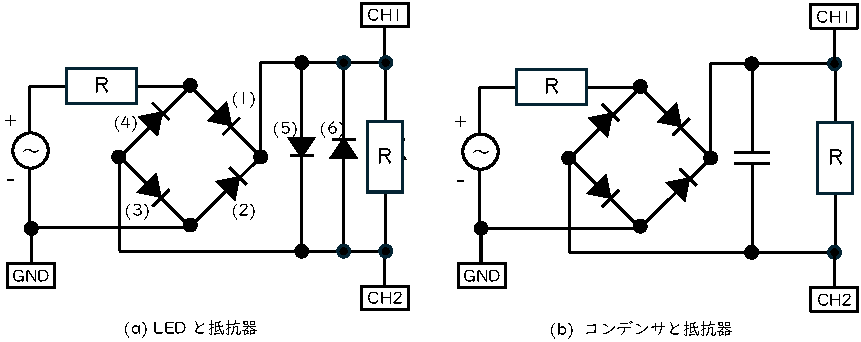
\includegraphics[width=0.95\linewidth]{diode_rectifier.pdf}
  \caption{整流回路}
  \label{fig:diode-rectifier}
\end{figure}

\begin{procedure}
  \item 図\ref{fig:diode-rectifier}(a)の回路をブレッドボード上に作製します。\wave{固定抵抗 \mbox{$R$} は\mbox{\SI{1}{\mega\ohm}}/\mbox{\SI{0.25}{W}}を使用します。}
  \item 交流電源をONにし，LEDの点灯状態を確認します。正電圧印加時にLED(1)，LED(3)，LED(5)が点灯し，負電圧印加時にLED(2)，LED(4)，LED(5)が点灯するため，正しく回路が接続されていれば，LED(1)，LED(3)，LED(5)とLED(2)，LED(4)，LED(5)が交互に点灯し，LED(6)は点灯しません。
  \item 確認後，交流電源の電源をOFFします。
  \item オシロスコープのCH1とCH2のプローブを図\ref{fig:diode-rectifier}(a)のように接続します。
  \item 「CH2」のボタンを押し，CH2を表示させ，CH2の電圧軸を\SI{2.00}{V}/DIVに設定します。
  \item 「Math」ボタンを押し，演算子を「$-$」に設定してCH1$-$CH2を表示させます。
  \item 「CH1」と「CH2」のボタンをそれぞれ2回押し，CH1とCH2の表示をOFFします。
  % 原文はSymbolフォントで「200 μs/DIV」。ms と判断（要確認）
  \item 交流電源をONして，オシロスコープで観察されるCH1$-$CH2のMathの電圧波形を課題2の図(b)に図示します。（オシロスコープの表示設定は\SI{2.00}{V}/DIV，\SI{200}{ms}/DIVのままです。）
  \item 図示後，交流電源をOFFします。
\end{procedure}

\subsubsection{整流回路2}

\begin{procedure}
  \item 図\ref{fig:diode-rectifier}(b)に示す回路をブレッドボード上に作製します。
  % 原文はSymbolフォントで「200 μs/DIV」。ms と判断（要確認）
  \item 交流電源をONにし，オシロスコープで観察されるCH1$-$CH2のMathの電圧波形を課題2の図(c)に図示します。（オシロスコープの表示設定は\SI{2.00}{V}/DIV，\SI{200}{ms}/DIVとします。）
  \item 図示後，交流電源をOFFにします。
\end{procedure}

\subsubsection{実験終了後}

\begin{procedure}
  \item オシロスコープの「Default Setup」ボタンを押し，オシロスコープの設定を初期化後，オシロスコープの電源をOFFします。
  \item オシロスコープと交流電源の電源ケーブルをはずします。また，実験に使用したLED，抵抗器，セラミックコンデンサーは袋にしまい，接続ケーブル等はプラスチックのケースに戻します。
\end{procedure}

% ============================================================
% トランジスタを用いた回路 本文
% 原本: トランジスタを用いた回路 20260727.docx
% 担当の先生はこのファイルと figures/ だけを編集してください。
% 図のラベルは fig:transistor-○○ の形にしてください（他テーマとの重複防止）。
% ============================================================
\graphicspath{{contents/04_transistor/figures/}}

\experimenttitle{トランジスタを用いた回路}

% ============================================================
\section{目的}

トランジスタは，小さな電気信号を用いてより大きな電流を制御できる電子素子であり，信号の増幅やスイッチングなど，さまざまな電子回路に広く利用されています。本実験では，トランジスタを用いてファンを駆動する回路を作製し，小さな入力によって負荷に流れる大きな電流を制御できることを確認します（\cref{fig:transistor-overview}）。さらに，入力電圧を変化させたときの電流や出力電圧を測定し，トランジスタの基本的な特性について理解します。

\begin{figure}[htbp]
  \centering
  \vspace{5mm}
  % 本実験の概要図（TikZ で作成。原本にはない図）
  \begin{tikzpicture}[
      font=\small,
      lbl/.style={font=\sffamily\gtfamily\small, align=center},
      small/.style={-latex, line width=0.6pt, EGMain!70},
      big/.style={-{Latex[length=3.2mm,width=3.2mm]}, line width=3pt, EGWarn!80},
    ]
    % ---- 入力：乾電池 ----
    \begin{scope}[shift={(0,0)}]
      \draw[fill=black!8, rounded corners=1pt] (-0.35,-0.75) rectangle (0.35,0.75);
      \fill[black!55] (-0.35,0.45) rectangle (0.35,0.75);
      \draw[fill=black!35] (-0.12,0.75) rectangle (0.12,0.88);
      \node at (0,0.0) {\scriptsize 1.5 V};
      \node[lbl] at (0,-1.55) {入力\\（乾電池）};
    \end{scope}
    % ---- トランジスタ ----
    \begin{scope}[shift={(4.2,0)}]
      \draw[fill=EGSub, draw=EGMain, rounded corners=3pt] (-1.1,-1.0) rectangle (1.1,1.0);
      \draw (0,0) node[npn, scale=1.2] (Q) {};
      \node[lbl] at (0,-1.55) {トランジスタ\\（増幅）};
    \end{scope}
    % ---- 負荷：ファン ----
    \begin{scope}[shift={(8.4,0)}]
      \draw[fill=black!8, rounded corners=4pt] (-0.9,-0.9) rectangle (0.9,0.9);
      \draw[fill=white] (0,0) circle (0.78);
      \foreach \a in {0,120,240}
        \fill[black!60, rotate=\a] (0,0) .. controls (0.25,0.15) and (0.55,0.45) .. (0.15,0.7)
                                          .. controls (0.05,0.45) and (-0.05,0.2) .. (0,0);
      \fill[black!80] (0,0) circle (0.14);
      \node[lbl] at (0,-1.55) {負荷\\（ファン）};
    \end{scope}
    % ---- ACアダプタ ----
    \node[draw, fill=black!8, rounded corners=2pt, lbl, minimum width=2.2cm, minimum height=0.8cm]
      (ac) at (8.4,2.5) {ACアダプタ（12 V）};
    % ---- 電流の矢印 ----
    \draw[small] (0.5,0) -- node[above, text=EGMain, font=\small] {小さな電流} (3.0,0);
    \draw[big] (ac.south) -- (8.4,0.95);
    \draw[big] (7.4,0) -- node[above=2pt, text=EGWarn, font=\small] {大きな電流} (5.4,0);
  \end{tikzpicture}
  \caption{本実験の概要（小さな入力でファンを駆動する）}
  \label{fig:transistor-overview}
\end{figure}

% ============================================================
\section{原理}

% ------------------------------------------------------------
\subsection{トランジスタとは？}

トランジスタは，さまざまな電気・電子機器に広く用いられている基本的な半導体素子で，
主な役割は「\important{増幅}」と「\important{スイッチング}」です。
増幅の例としては，音声信号を大きくするオーディオアンプや，センサから得られる微弱な信号を扱いやすい大きさにする回路などがあります。
スイッチングの例としては，コンピュータの中央処理装置（CPU：Central Processing Unit）やメモリなどのデジタル回路があり，そこでは集積された数十億個以上のトランジスタが高速にオン・オフを繰り返すことで情報処理を行っています。
また，電源回路やモータ駆動回路などでも，精密な制御基盤との絶縁を保ちながら大電流・大電力を制御するためにトランジスタが広く利用されています。
このようにトランジスタは「電気信号や電力を制御する素子」として，さまざまな電気・電子機器の心臓部を担っています。

% ------------------------------------------------------------
\subsection{トランジスタの種類}

トランジスタは，大きく「\important{バイポーラトランジスタ（BJT：Bipolar Junction Transistor）}」と「\important{電界効果トランジスタ（FET：Field-Effect Transistor）}」に分類され，動作原理や特性に違いがあります。
\wave{本実験では，これら2種類のトランジスタのうち，BJTを扱います}。

\vspace{5mm}

% BJT と FET の図と説明を左右2つの枠に並べる（枠の高さはそろえる）
\noindent
\begin{minipage}[t]{0.49\linewidth}
\begin{tcolorbox}[enhanced, equal height group=transistor-types, colback=white, colframe=EGMain,
    boxrule=0.6pt, arc=1mm, left=2mm, right=2mm, top=2mm, bottom=2mm,
    fonttitle=\sffamily\gtfamily\bfseries, toptitle=1mm, bottomtitle=1mm,
    coltitle=white, colbacktitle=EGMain, title={バイポーラトランジスタ（BJT）}]
\begin{center}
  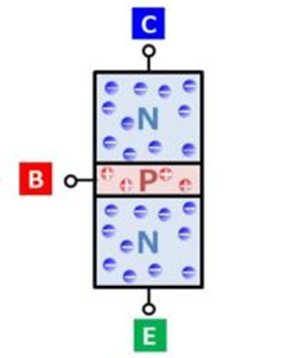
\includegraphics[height=32mm]{transistor_npn_structure.png}\hspace{5mm}
  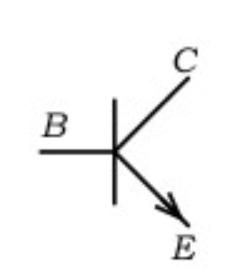
\includegraphics[height=24mm]{transistor_npn_symbol.png}
  \captionof{figure}{バイポーラトランジスタ（BJT）}
  \label{fig:transistor-bjt}
\end{center}
BJTは，ベース（B），コレクタ（C），エミッタ（E）の3つの端子を持つトランジスタです（\cref{fig:transistor-bjt}）。
ベースに流す小さな電流によって，コレクタとエミッタの間に流れる大きな電流を制御することから，「\important{電流で電流を制御する素子}」と考えることができます。
小さな入力に対して大きな電流変化を得やすく，音声信号やセンサ信号などを扱うアナログ増幅回路で用いられることが多いトランジスタです。
また，小型モータの駆動や速度制御などにも利用されます。
\end{tcolorbox}
\end{minipage}\hfill
\begin{minipage}[t]{0.49\linewidth}
\begin{tcolorbox}[enhanced, equal height group=transistor-types, colback=white, colframe=EGMain,
    boxrule=0.6pt, arc=1mm, left=2mm, right=2mm, top=2mm, bottom=2mm,
    fonttitle=\sffamily\gtfamily\bfseries, toptitle=1mm, bottomtitle=1mm,
    coltitle=white, colbacktitle=EGMain, title={電界効果トランジスタ（FET）}]
\begin{center}
  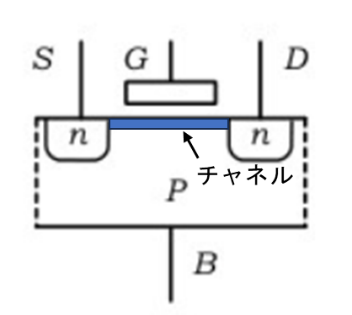
\includegraphics[height=32mm]{transistor_fet_structure.png}
  \captionof{figure}{電界効果トランジスタ（FET）}
  \label{fig:transistor-fet}
\end{center}
FETは，ゲート（G），ドレイン（D），ソース（S）の3つの端子を持つトランジスタです（\cref{fig:transistor-fet}）。
ゲートに加える電圧によって，ドレインとソースの間に流れる電流を制御することから，「\important{電圧で電流を制御する素子}」と考えることができます。
入力側に流れる電流が非常に小さく，小型化や高集積化にも適していることから，CPUやメモリなどのデジタル回路に広く用いられています。
また，大きな電力を扱う電源回路のスイッチングにも多く利用されています。
\end{tcolorbox}
\end{minipage}

% ------------------------------------------------------------
\subsection{バイポーラトランジスタの基本的な性能}

本実験ではBJTを扱っていきます。BJTは主にPNP型とNPN型があり，ここではNPN型について説明します。NPN型のトランジスタは，\cref{fig:transistor-bjt}のような記号で表され，ベース（B）に小さな電流を流すことで，エミッタ（E）からコレクタ（C）へ流れる大きな電流を制御できる素子です。すなわち「小さい入力電流で大きな出力電流を操る」増幅作用を持ちます。

NPN型では，ベース-エミッタ間に電圧（約\SI{0.7}{V}以上）を与えると，エミッタからベースへ電子が流れ込みます。ベースは非常に薄いため，その電子の一部のみが正孔と再結合してベース電流となり，残りのほとんどの電子はそのままコレクタへ引き抜かれます（コレクタ電流）。この結果，小さなベース電流に対して大きなコレクタ電流が流れます。この関係は $I_\mathrm{C}=\beta I_\mathrm{B}$（$\beta$ は電流増幅率）で表され，$\beta$ は一般に数十から数百の値をとります。また，コレクタ-エミッタ間に適切な電圧を与えることで，トランジスタはアナログ信号の増幅素子としてだけでなく，デジタル回路におけるスイッチとしても利用されます。

% ------------------------------------------------------------
\subsection{エミッタ接地増幅回路}

\begin{figure}[htbp]
  \centering
  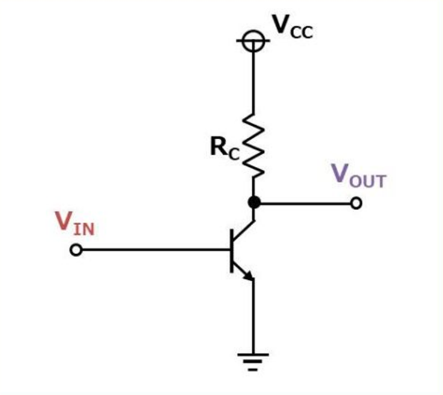
\includegraphics[height=45mm]{transistor_ce_amplifier.png}
  \caption{エミッタ接地増幅回路}
  \label{fig:transistor-ce}
\end{figure}

エミッタ接地増幅回路は，エミッタ端子を接地（GND）に接続し，ベースに直流電圧を加えてコレクタ電流を制御する回路です（\cref{fig:transistor-ce}）。ベース−エミッタ間にはおよそ\SI{0.7}{V}程度の電圧が必要であり，このとき流れるベース電流に比例してコレクタ電流が流れます。コレクタ電流が大きくなるとコレクタ抵抗にかかる電圧降下も大きくなり，その結果コレクタ電圧（$V_\mathrm{OUT}$）は低下します。このように入力側のベース電圧を変化させると，出力側のコレクタ電圧が反対方向に変化するため「反転動作」と呼ばれます。直流の実験では，この電圧−電流関係やコレクタ電圧の変化を測定し，トランジスタの基本特性と動作点の決まり方を確認できます。

% ============================================================
\section{実験}

結果は，ワークシートに記入してください。

% ------------------------------------------------------------
\subsection{実験1：乾電池（小さな入力信号）を用いてファンを回そう！}

\begin{equipment}[準備物]
ブレッドボード，ジャンパー線，ファン（\SI{12}{V}），乾電池（\SI{1.5}{V}），電池BOX，DCジャック，トランジスタ，ACアダプタ（\SI{12}{V}），抵抗（\SI{1}{k\ohm}）
\end{equipment}

\begin{figure}[htbp]
  \centering
  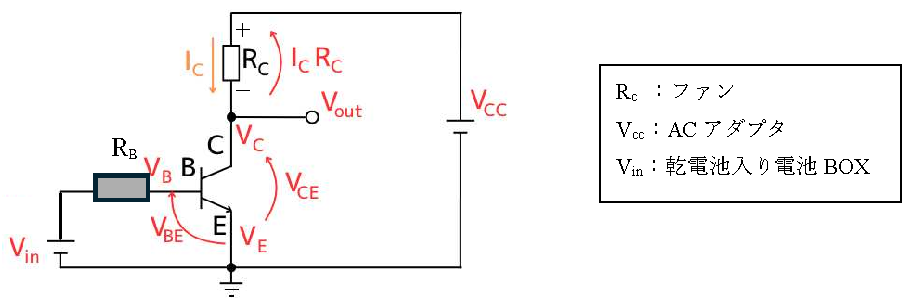
\includegraphics[width=0.95\linewidth]{transistor_fan_circuit.pdf}
  \caption{ファン駆動用エミッタ接地増幅回路}
  \label{fig:transistor-fan}
\end{figure}

\begin{figure}[htbp]
  \centering
  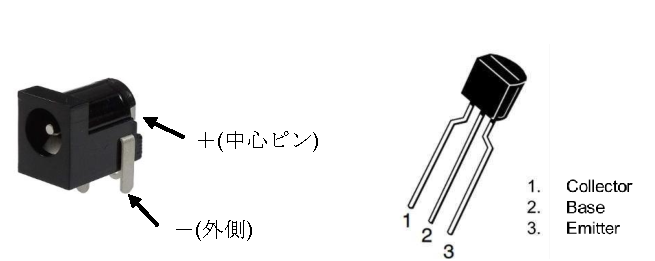
\includegraphics[width=0.7\linewidth]{transistor_dcjack_pinout.pdf}
  \caption{本実験で使用するDCジャックとトランジスタ}
  \label{fig:transistor-dcjack}
\end{figure}

\begin{procedure}[label=\textbf{1.\arabic*}, ref=1.\arabic*, leftmargin=*, labelsep=0.8em]
  \item ブレッドボード上で，乾電池入り電池BOXとファンを直列に接続し，ファンが駆動するか確認します。回ったかどうかをワークシートに記入してください。
  \item 乾電池でファンを回してみます。\cref{fig:transistor-fan}の回路図のように，ブレッドボード上に増幅回路を組み立てます。このときの $R_\mathrm{c}$ はファン，$V_\mathrm{cc}$ はACアダプタ，$V_\mathrm{in}$ は乾電池入り電池BOXです。\wave{トランジスタのエミッタ，コレクタ，ベースの各端子，およびDCジャックの極性（$+$・$-$）を，\cref{fig:transistor-dcjack}を参考にして正しく接続します。}
  \item 接続を確認した後，電池BOXのスイッチをオンにし，増幅回路を用いてファンを駆動します。\wave{ファンが回転したら教員の確認を受け}，実験2に進みます。
\end{procedure}

% ------------------------------------------------------------
\subsection{実験2：電圧−電流の関係やコレクタ電圧の変化を測定しよう！}

\begin{equipment}[準備物]
ブレッドボード，ジャンパー線，ファン（\SI{12}{V}），DCジャック，トランジスタ，ACアダプタ（\SI{12}{V}），抵抗（\SI{1}{k\ohm}×2個），直流電源，テスター
\end{equipment}

\begin{procedure}[label=\textbf{2.\arabic*}, ref=2.\arabic*, leftmargin=*, labelsep=0.8em]
  \item ファンが回り始める入力電圧のしきい値を確認します。増幅回路の入力電圧源 $V_\mathrm{in}$ を乾電池から直流電源に変更します。$V_\mathrm{in}$ を\SI{0}{V}から\SI{1.0}{V}まで\SI{0.05}{V}ずつ上昇させ，ファンが回り始めたときの電圧をワークシートに記録します。
  \item \label{item:transistor-graph} ファンを\SI{1}{k\ohm}のコレクタ抵抗 $R_\mathrm{c}$ に置き換え，抵抗の両端電圧 $V_{R_\mathrm{c}}$ をテスターで測定します。$V_\mathrm{in}$ を\SI{0}{V}から\SI{1.0}{V}まで\SI{0.05}{V}ずつ変化させ，横軸を $V_\mathrm{in}$，縦軸を $V_{R_\mathrm{c}}$ としてグラフを作成します。
  \item 出力電圧 $V_\mathrm{OUT}$ を，コレクタ端子とGNDとの間の電圧として測定します。$V_\mathrm{in}$ を\SI{0}{V}から\SI{1.0}{V}まで\SI{0.05}{V}ずつ変化させ，横軸を $V_\mathrm{in}$，縦軸を $V_\mathrm{OUT}$ として，\ref{item:transistor-graph}で作成したグラフ上にプロットします。
\end{procedure}

% ============================================================
% 電圧波の観測 本文
% 原本: 伝送線路_改v2.docx（である調 → です・ます調に変更）
% 担当の先生はこのファイルと figures/ だけを編集してください。
% 図のラベルは fig:voltagewave-○○ の形にしてください（他テーマとの重複防止）。
% ============================================================
\graphicspath{{contents/05_voltagewave/figures/}}

\experimenttitle{電圧波の観測}

% ============================================================
\section{目的}

電気信号伝搬の現象を観察し，理解を深めます。

% ============================================================
\section{原理}

\subsection{電気信号の伝搬}

基本的に真空中では電気信号は光速 $c$ と同等の $\SI{3e8}{m/s}$ で移動します。しかし一般的に電気信号は比誘電率をもつ絶縁体の中を移動することが多く，その伝搬速度 $v$ はその実効比誘電率 $\varepsilon_\mathrm{r}$ と光速 $c$ から
\begin{equation}
  v = \frac{c}{\sqrt{\varepsilon_\mathrm{r}}}
  \label{eq:voltagewave-velocity}
\end{equation}
と求めることができます。電気信号は速度を持つことから，電気信号が伝わる線（伝送線路）の長さによって信号の到達時間も変化します。

交流電源は電圧波高値と周波数があり，周波数 $f$（Hz）は1秒当たりの波の数であり，その逆数は周期 $T$（s）です。
\begin{equation}
  T = \frac{1}{f}
  \label{eq:voltagewave-period}
\end{equation}

% ============================================================
\section{使用器具}

\begin{equipment}
\begin{itemize}
  % TODO(原文確認): ファンクションジェネレータが「1台/部屋」と「1台/班」の2行ある
  \item ファンクションジェネレータ（1台/部屋）
  \item ファンクションジェネレータ（1台/班）
  \item ディジタルオシロスコープ \SI{50}{MHz}（1台/班）
  \item 同軸ケーブル（1本/班）
  \item BNC T字分岐コネクタ（1個/班）
  \item 終端抵抗（1個/班）
\end{itemize}
\end{equipment}

% ============================================================
\section{実験方法}

【　】の部分には，実験で得られた値を記入してください。

% ------------------------------------------------------------
\subsection{実験1：電気信号の進む速さを見てみよう！}

\begin{figure}[htbp]
  \centering
  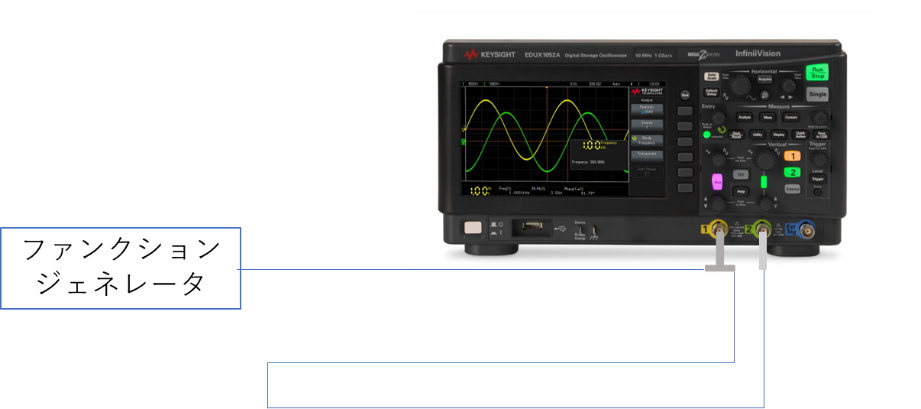
\includegraphics[width=0.75\linewidth]{voltagewave_circuit1.png}
  \caption{実験回路1}
  \label{fig:voltagewave-circuit1}
\end{figure}

\begin{procedure}[label=\textbf{(\arabic*)}, ref=(\arabic*), leftmargin=*, labelsep=0.8em]
  \item オシロスコープのch1にBNC T字分岐コネクタを，ch2に※終端抵抗を接続します。\cref{fig:voltagewave-circuit1}のようにファンクションジェネレータ出力端とオシロスコープch1のT字分岐コネクタの一端を同軸ケーブルで接続します。T字分岐コネクタのもう一端とオシロスコープのch2を長さ【　　　　】mの同軸ケーブル（RG-58A/U）で接続します。
  \item ファンクションジェネレータの電源を入れます。
  \item ファンクションジェネレータの出力を矩形波に設定して周波数を【　　　　】Hzにします。
  \item 信号の時間のずれが発生するようにオシロスコープの時間軸を【　　　　】s/Divに調整し，時間のずれを観測します。\\
    測定結果：時間のずれ【　　　　】s
  \item 観測した時間から電気信号の進む速さを算出します。\\
    計算結果：電気信号伝搬速度【　　　　】m/s
\end{procedure}

※SI接頭語（大きな数字を表すのに便利な文字）を使って適切に表しましょう（\cref{tab:voltagewave-prefix}）。

\begin{table}[htbp]
  \centering
  \caption{SI接頭語}
  \label{tab:voltagewave-prefix}
  \begin{tabular}{ccccccc}
    \toprule
    ナノ & マイクロ & ミリ & & キロ & メガ & ギガ \\
    n & μ & m & & k & M & G \\
    $10^{-9}$ & $10^{-6}$ & $10^{-3}$ & & $10^{3}$ & $10^{6}$ & $10^{9}$ \\
    \bottomrule
  \end{tabular}
\end{table}

% ------------------------------------------------------------
\subsection{実験2：定在波を見てみよう！}

\begin{figure}[htbp]
  \centering
  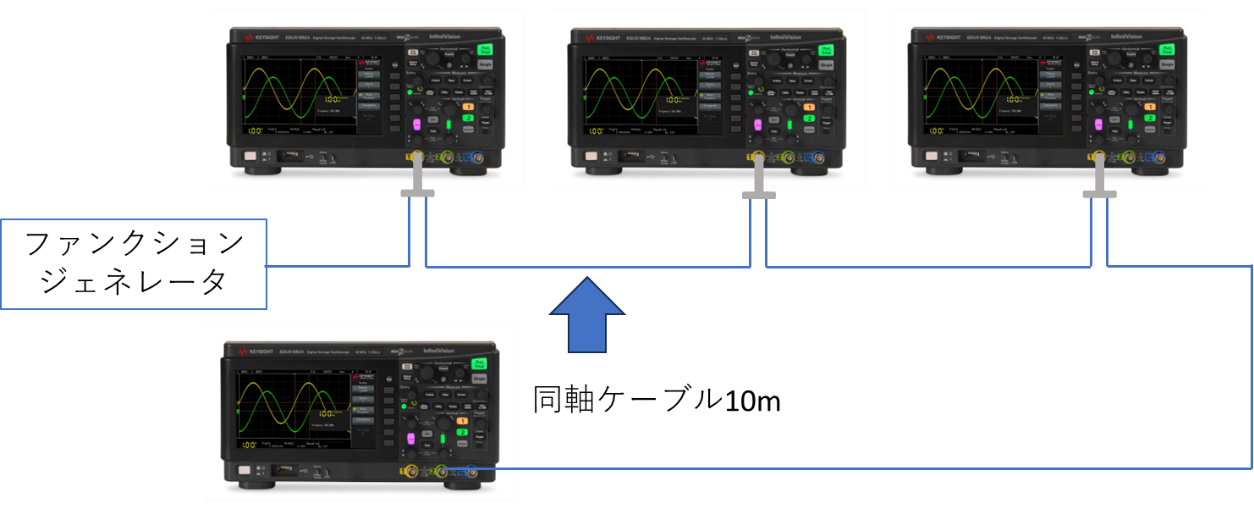
\includegraphics[width=0.9\linewidth]{voltagewave_circuit2.png}
  \caption{実験回路2}
  \label{fig:voltagewave-circuit2}
\end{figure}

\begin{procedure}[label=\textbf{(\arabic*)}, ref=(\arabic*), leftmargin=*, labelsep=0.8em]
  \item 実験1でファンクションジェネレータにつないでいたBNCケーブルを外します。
  \item オシロスコープのch2に接続していた同軸ケーブルの端子を\cref{fig:voltagewave-circuit2}のように他の班のオシロスコープの送電端（ch1）に接続し，部屋で1つのケーブルになるように接続します。
  \item 各班の同軸ケーブルの長さを表2に記録します。
  \item \label{item:voltagewave-freq} 各班の線の長さの合計【　　　　】mが波長になる周波数【　　　　】Hzを算出します。
  \item \label{item:voltagewave-table2} ファンクションジェネレータの電源を入れ，電圧値\SI{2}{V}，周波数\SI{100}{kHz}に設定し，周波数を徐々に上げます。電圧値が初めて\SI{0.5}{V}を下回った位置の同軸ケーブル長を記録します。そのときの各オシロスコープの電圧値を表2に記録します。\\
    同軸ケーブル長【　　　　】m
  % 原文は「（3）で求めた値」だが，周波数を求めるのは（4）なので参照を修正
  \item \label{item:voltagewave-table3} 周波数を\ref{item:voltagewave-freq}で求めた値まで上げた際の各班のオシロスコープの最大電圧値を表3に記録します。
\end{procedure}


\end{document}
